% Appendix A

\chapter{Appendix} % Main appendix title

\label{AppendixA} % For referencing this appendix elsewhere, use \ref{AppendixA}

%-----------------------------------
%	SECTION Python code
%-----------------------------------
\vspace{\baselineskip}
\vspace{\baselineskip}

\section{Glossary}
    \subsection{French}
        Acompte [\textit{Advance}] : paiement partiel à valoir sur le montant d'une somme due.\\
        AR [\textit{Back}] : arrière.\\
        Armoire [\textit{Cabinet}] : meuble permettant de stocker différents objets.\\
        AV [\textit{Front}] : avant.\\
        Casier [\textit{Storage box}] : sous partie de l’armoire. \\
        Clôturer [\textit{Close}] : finaliser, terminer une commande. \\
        Cornière [\textit{Angle}] : pièce verticale formant les coins de l’armoire. \\
        Coupelle [\textit{Knop}] : pièce de plastique placé sur la porte permettant d’agripper la porte et de la déplacer facilement. \\
        Facture [\textit{Bill-Invoice}] : pièce comptable par laquelle le vendeur fait connaître à l'acheteur le détail et le prix des marchandises vendues et services exécutés. \\
        Fournisseur [\textit{Supplier}] : personne/société qui fournit des marchandises de façon habituelle. \\
        GD [\textit{Left/Right}] : gauche - droite.\\
        HB [\textit{Up/Down}] : haut - bas.\\
        Magasinier [\textit{Storekeeper}] : employé s’occupant du magasin, du stock et des clients. \\
        Panneau [\textit{Panel}] : plaque de bois formant les parois de l’armoire.\\
        Parois [\textit{side}] :  côtés de l’armoire. \\
        Porte [\textit{Door}] : parois de bois ou de verre permettant de fermer le casier. \\
        Rainure [\textit{Groove}] : entaille longue dans une pièce permettant de faire passer la porte et de pouvoir la coulisser. \\
        Standardisées [\textit{Standardized}] : adjectif donner à un produit, une production à une norme, à un modèle unique. \\
        Tablettes [\textit{Shelf}] : plaque horizontale sur laquelle on peut poser divers objets. \\
        Tasseau [\textit{Cleat}] : petite pièce de bois destinée à soutenir l'extrémité d’un panneau. \\
        Tiroir [\textit{Drawer}] : Compartiment ouvert sur le haut, glissé dans un meuble. \\
        Traverse [\textit{Beam/Tie}] : pièce horizontale faisant partie de l’armature (arêtes) de l’armoire.
    
    \newpage
    \subsection{English}
        Advance [\textit{Acompte}]: partial payment on a total sum due.  \\
        Angle [\textit{Cornière}]: vertical part strengthening the cabinet’s corners. \\
        Back [\textit{AR}] \\
        Beam/Tie [\textit{Travèrse}]: horizontal part of the cabinet. It gives its strength to the cabinet. \\
        Bill [\textit{Facture}]: Accounting document by which the seller informs the buyer of the details and the price of the goods sold and services executed. \\
        Cabinet [\textit{Armoire}]: furniture to stock different objects. \\
        Cleat [\textit{Tasseau}]: small part made of wood supporting the extremity of a panel. \\
        Close [\textit{Clôturer}]: finalize, end an order.  \\
        Door [\textit{Porte}]: Wooden or glass plate allowing the storage box to be closed. 
        Down [\textit{HB}] \\
        Drawer [\textit{Tiroir}]: compartment opens on the upper side, slid into furniture. \\ 
        Front [\textit{AV}] \\
        Groove [\textit{Rainure}]: long cut in a part to place a sliding door. \\
        Invoice [\textit{Facture}]: Accounting document by which the seller informs the buyer of the details and the price of the goods sold and services executed. \\
        Knop [\textit{Coupelle}]: plastic part placed on the door to move it easier. \\
        Left [\textit{GD}] \\
        Panel [\textit{Panneau}]: wooden plate forming the cabinet’s wall. \\
        Right [\textit{GD}] \\
        Shelf [\textit{Tablette}]: horizontal plate to place objects. \\
        Side [\textit{Parois}]: cabinet or storage box wall. \\
        Standardized [\textit{Standardisée}]: adjective given to a product, a production with a norm or a unique model. \\
        Storage box [\textit{Casier}]: subpart of the cabinet. \\
        Storekeeper [\textit{Magasinier}]: Employee managing the store, the stock and the customers. \\
        Supplier [\textit{Fournisseur}]: person or company supplying regularly the commodity.\\ 
        Up [\textit{HB}]
%-----------------------------------
%	SECTION Python code
%-----------------------------------



\newpage
\section{Diagrams}
\label{diagrams}
    \subsection{Activity Diagram}
        \vfill
        \begin{figure*}[h!]
            \centering
			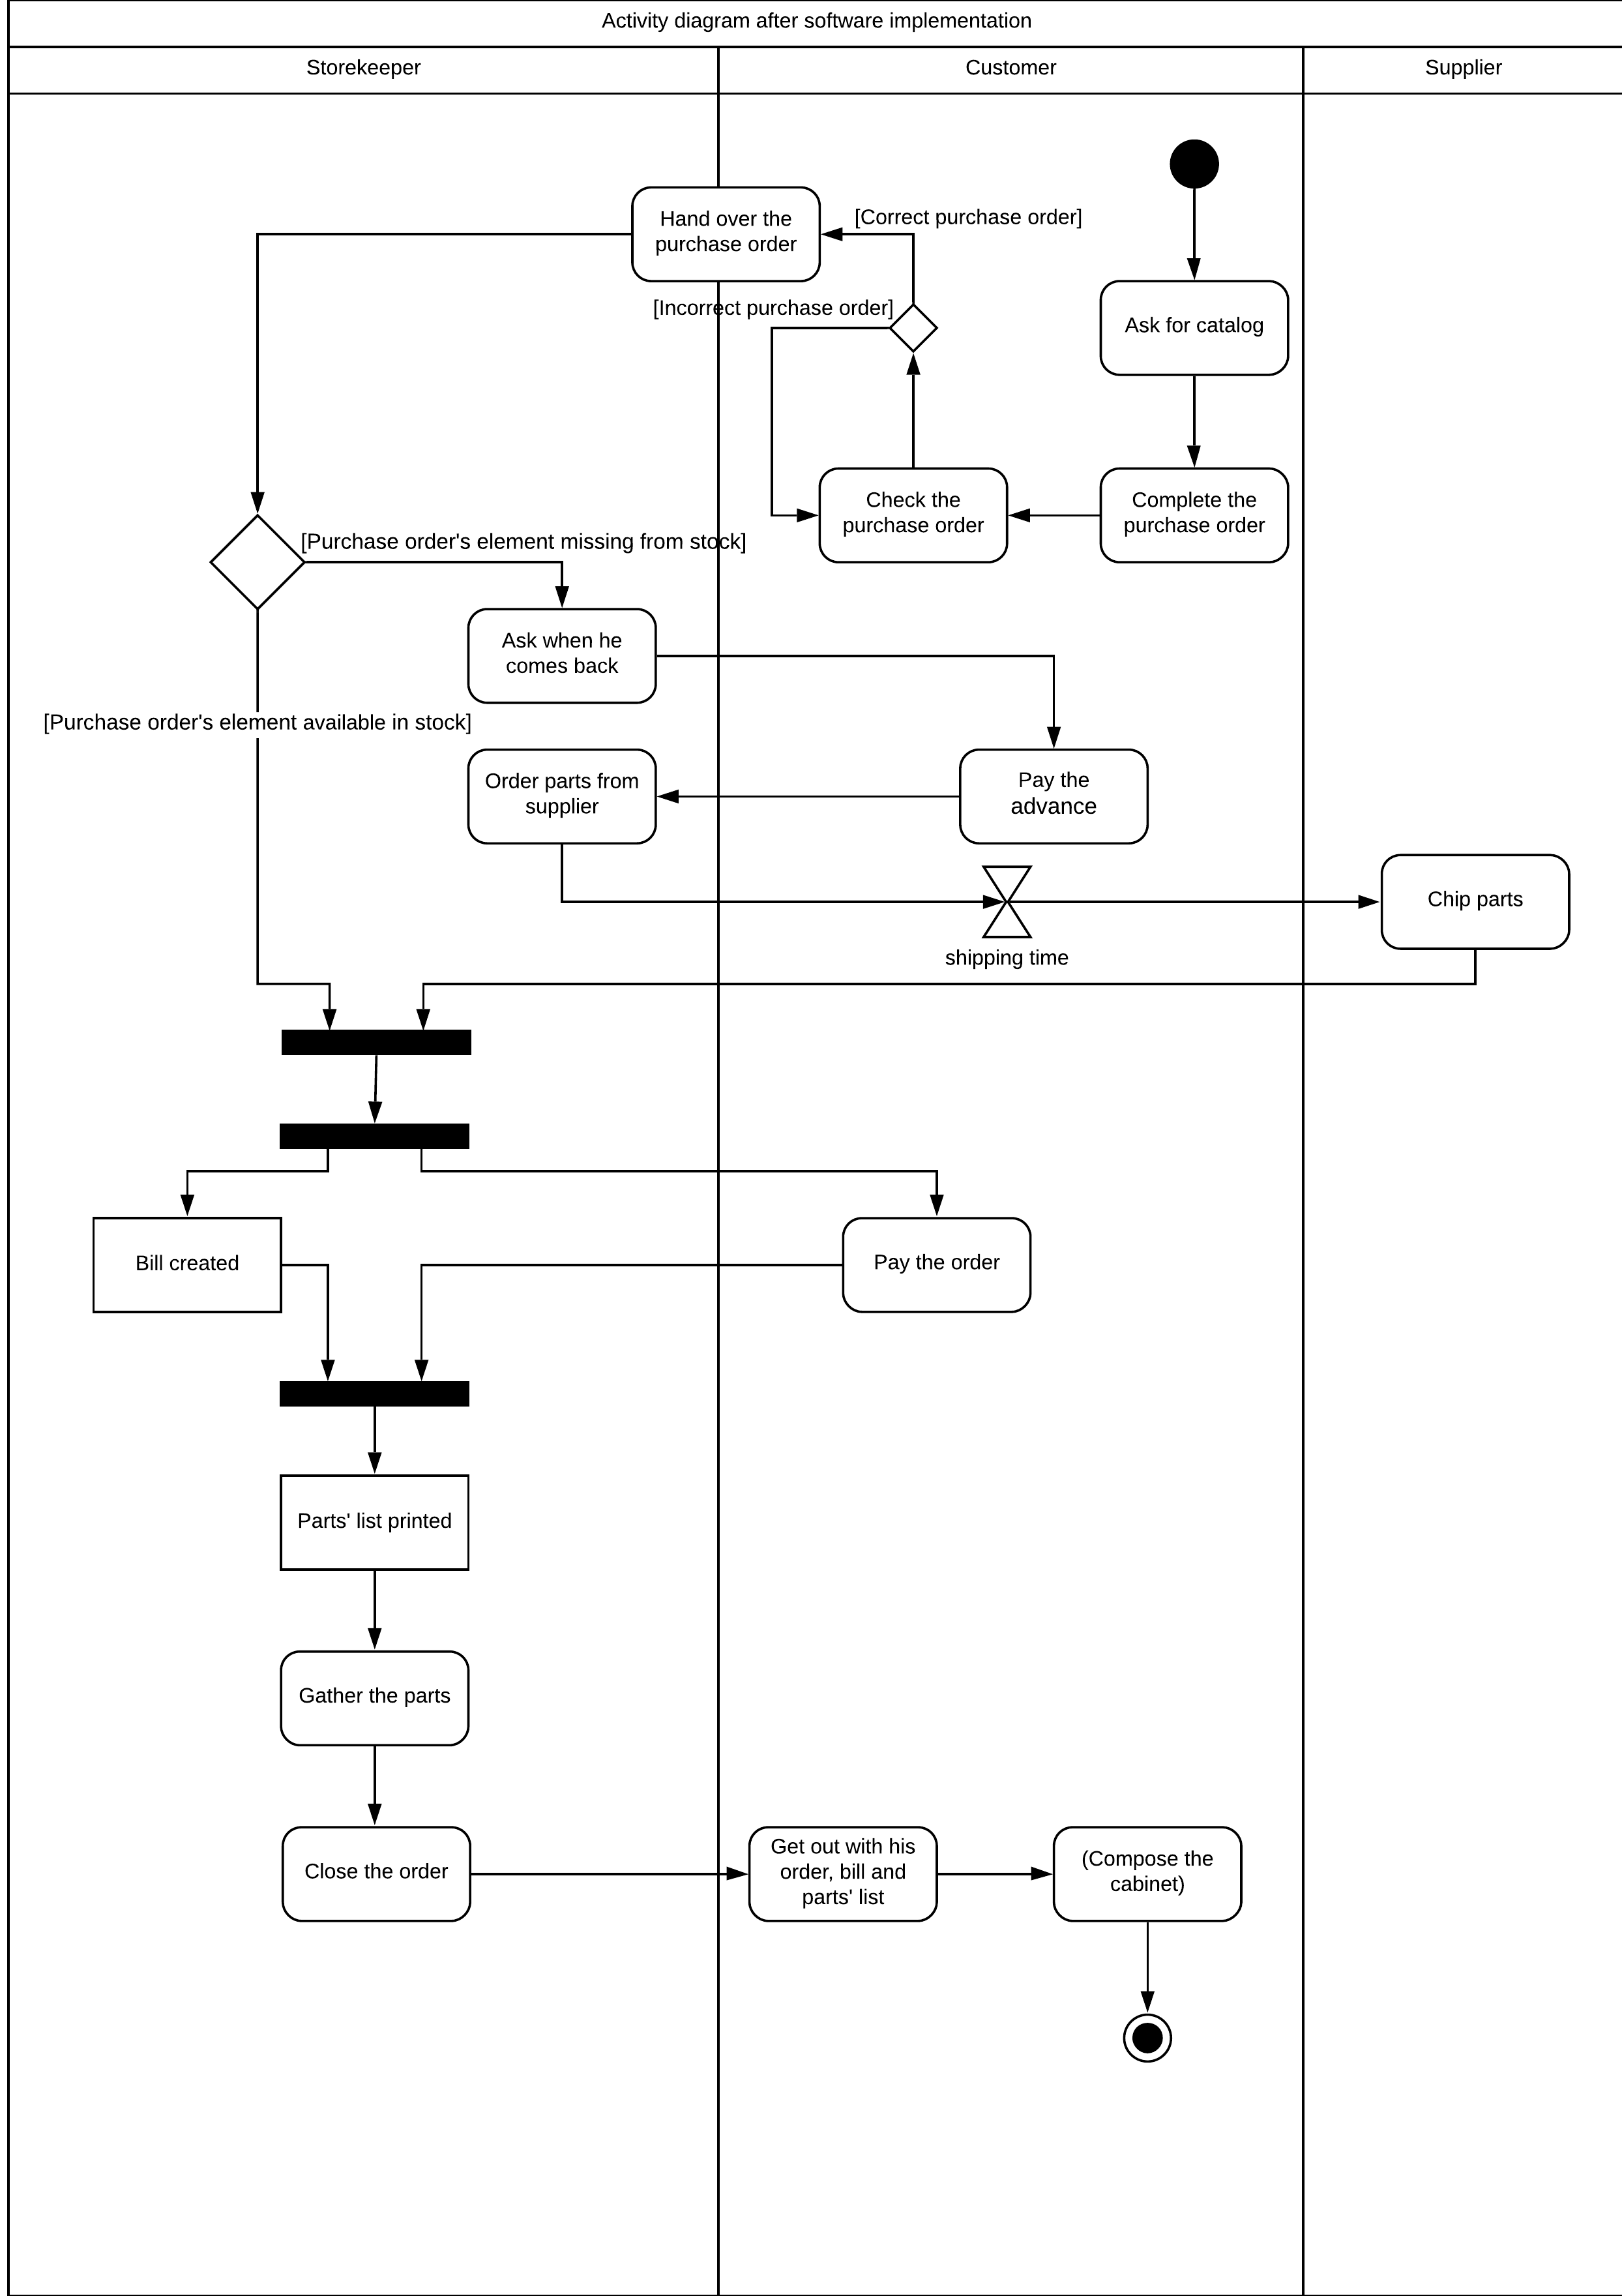
\includegraphics[width =0.8\textwidth]{Figures/ActivityDiagram.png}
			\rule{35em}{0.5pt}
			\caption{Activity Diagram}
			\label{activitydiagram}
    	\end{figure*}
        \vfill
        
    \newpage
    \subsection{Activity Standard Dimension Diagram}
        \vfill
        \begin{figure*}[h!]
            \centering
			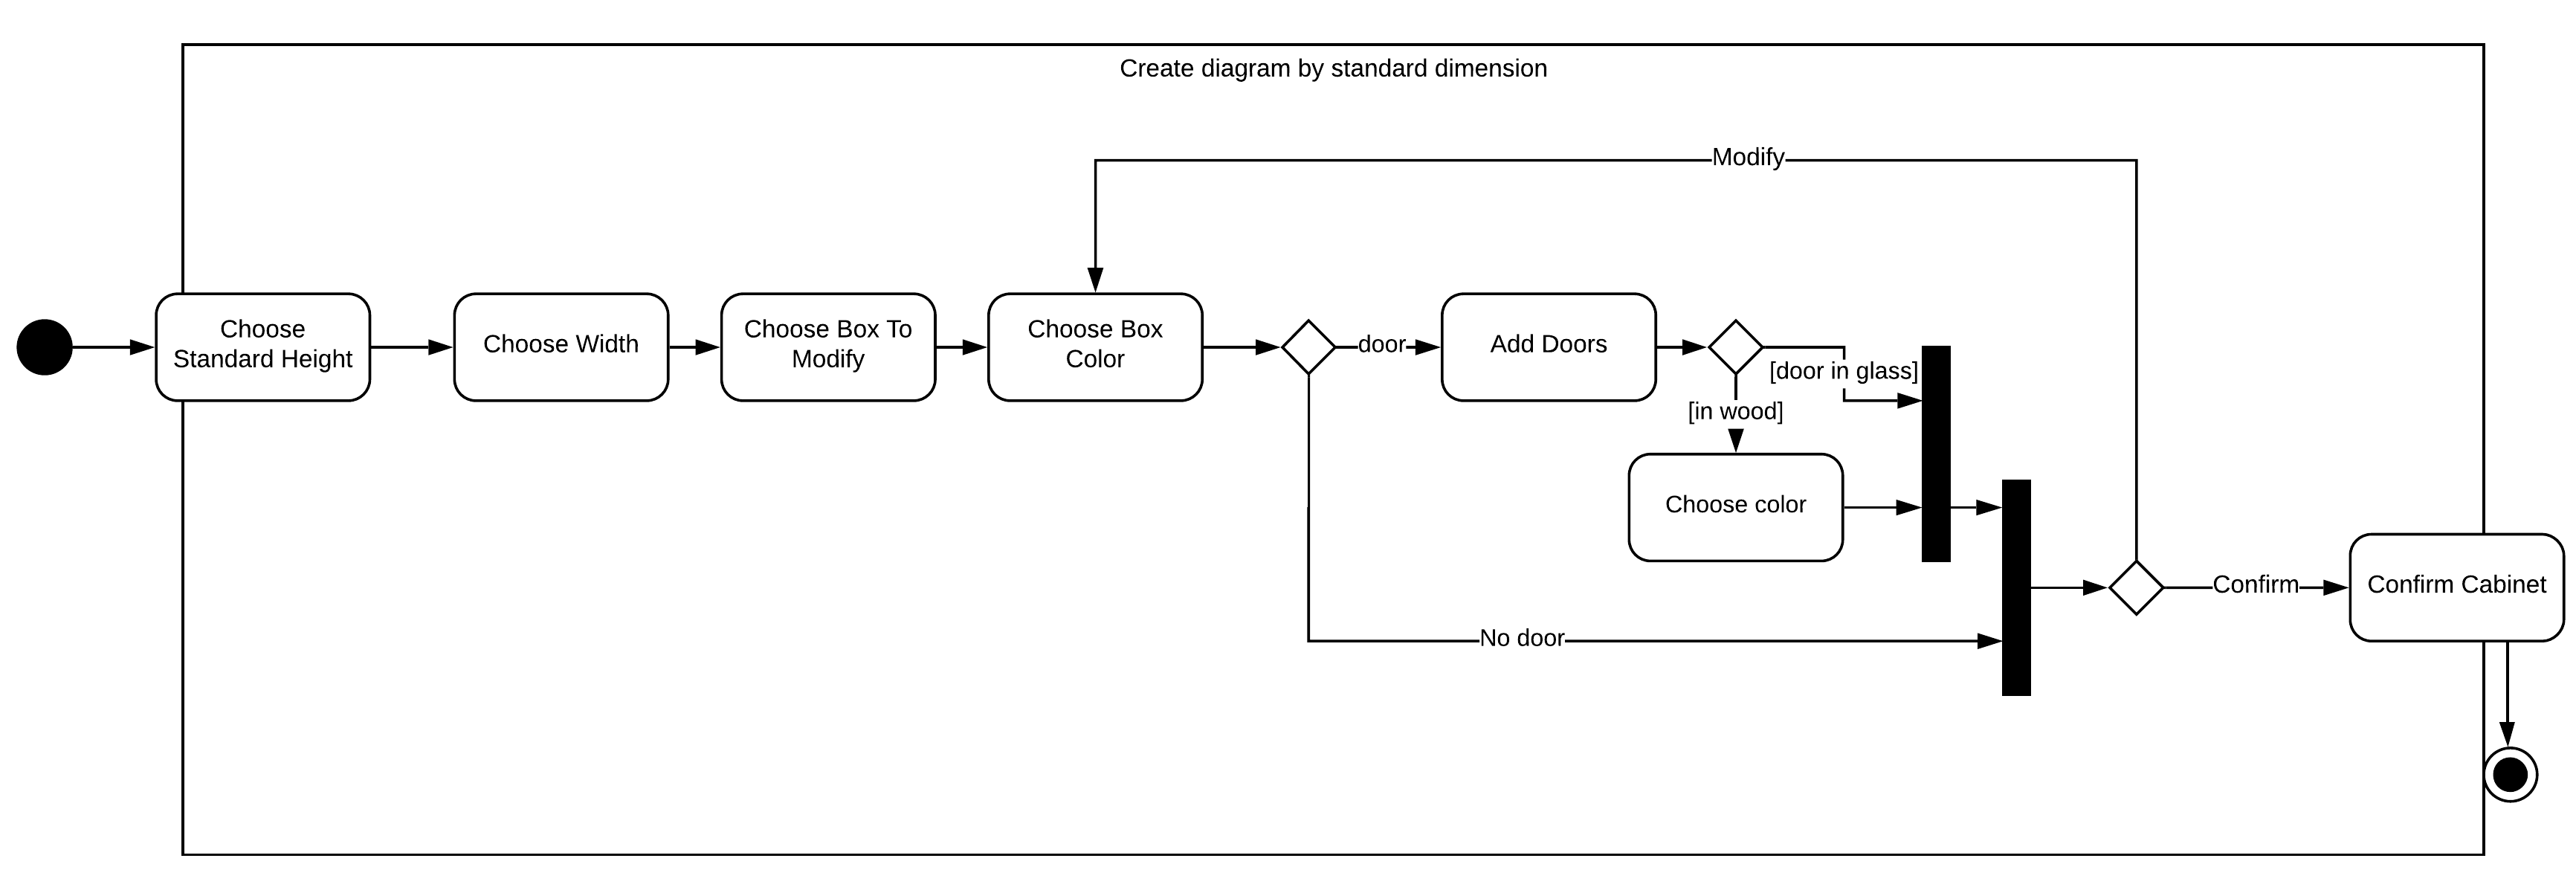
\includegraphics[angle = 90, height=185mm]{Figures/ActivityStandardDiagram.png}
			\rule{35em}{0.5pt}
			\caption{Activity Standard Dimension Diagram}
			\label{activitystandartdiagram}
    	\end{figure*}
        \vfill
        
    \newpage
    \subsection{Activity Cabinet Creation Diagram}
        \vfill
        \begin{figure*}[h!]
            \centering
			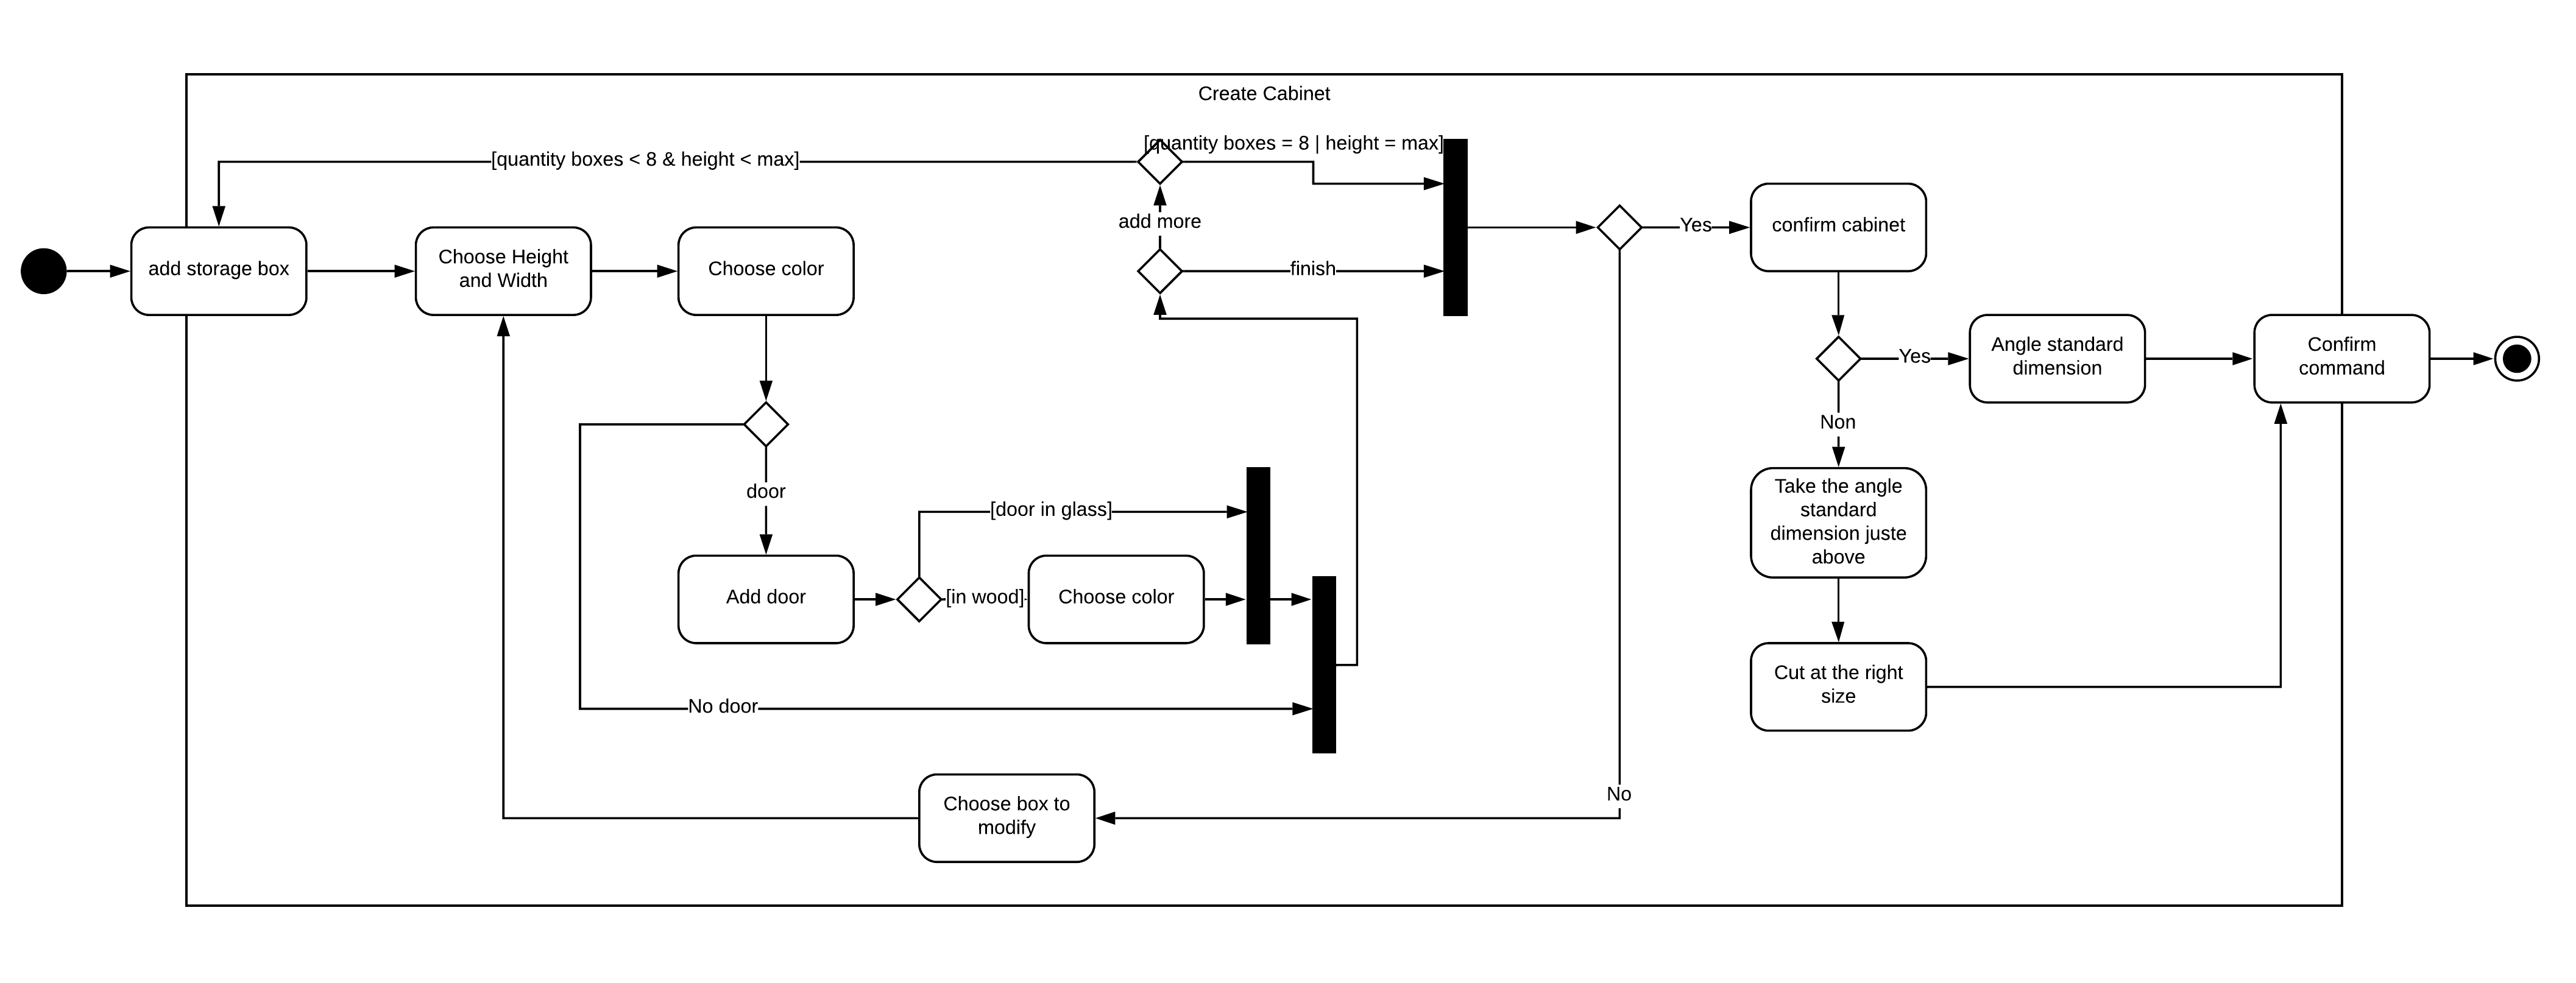
\includegraphics [angle = 90, height=185mm]{Figures/ActivityCabinetDiagram.png}
			\rule{35em}{0.5pt}
			\caption{Activity Cabinet Creation Diagram}
			\label{activitycabinetdiagram}
    	\end{figure*}
        \vfill
        
    \newpage
    \subsection{Use Case Diagram}
        \vfill
        \begin{figure*}[h!]
            \centering
			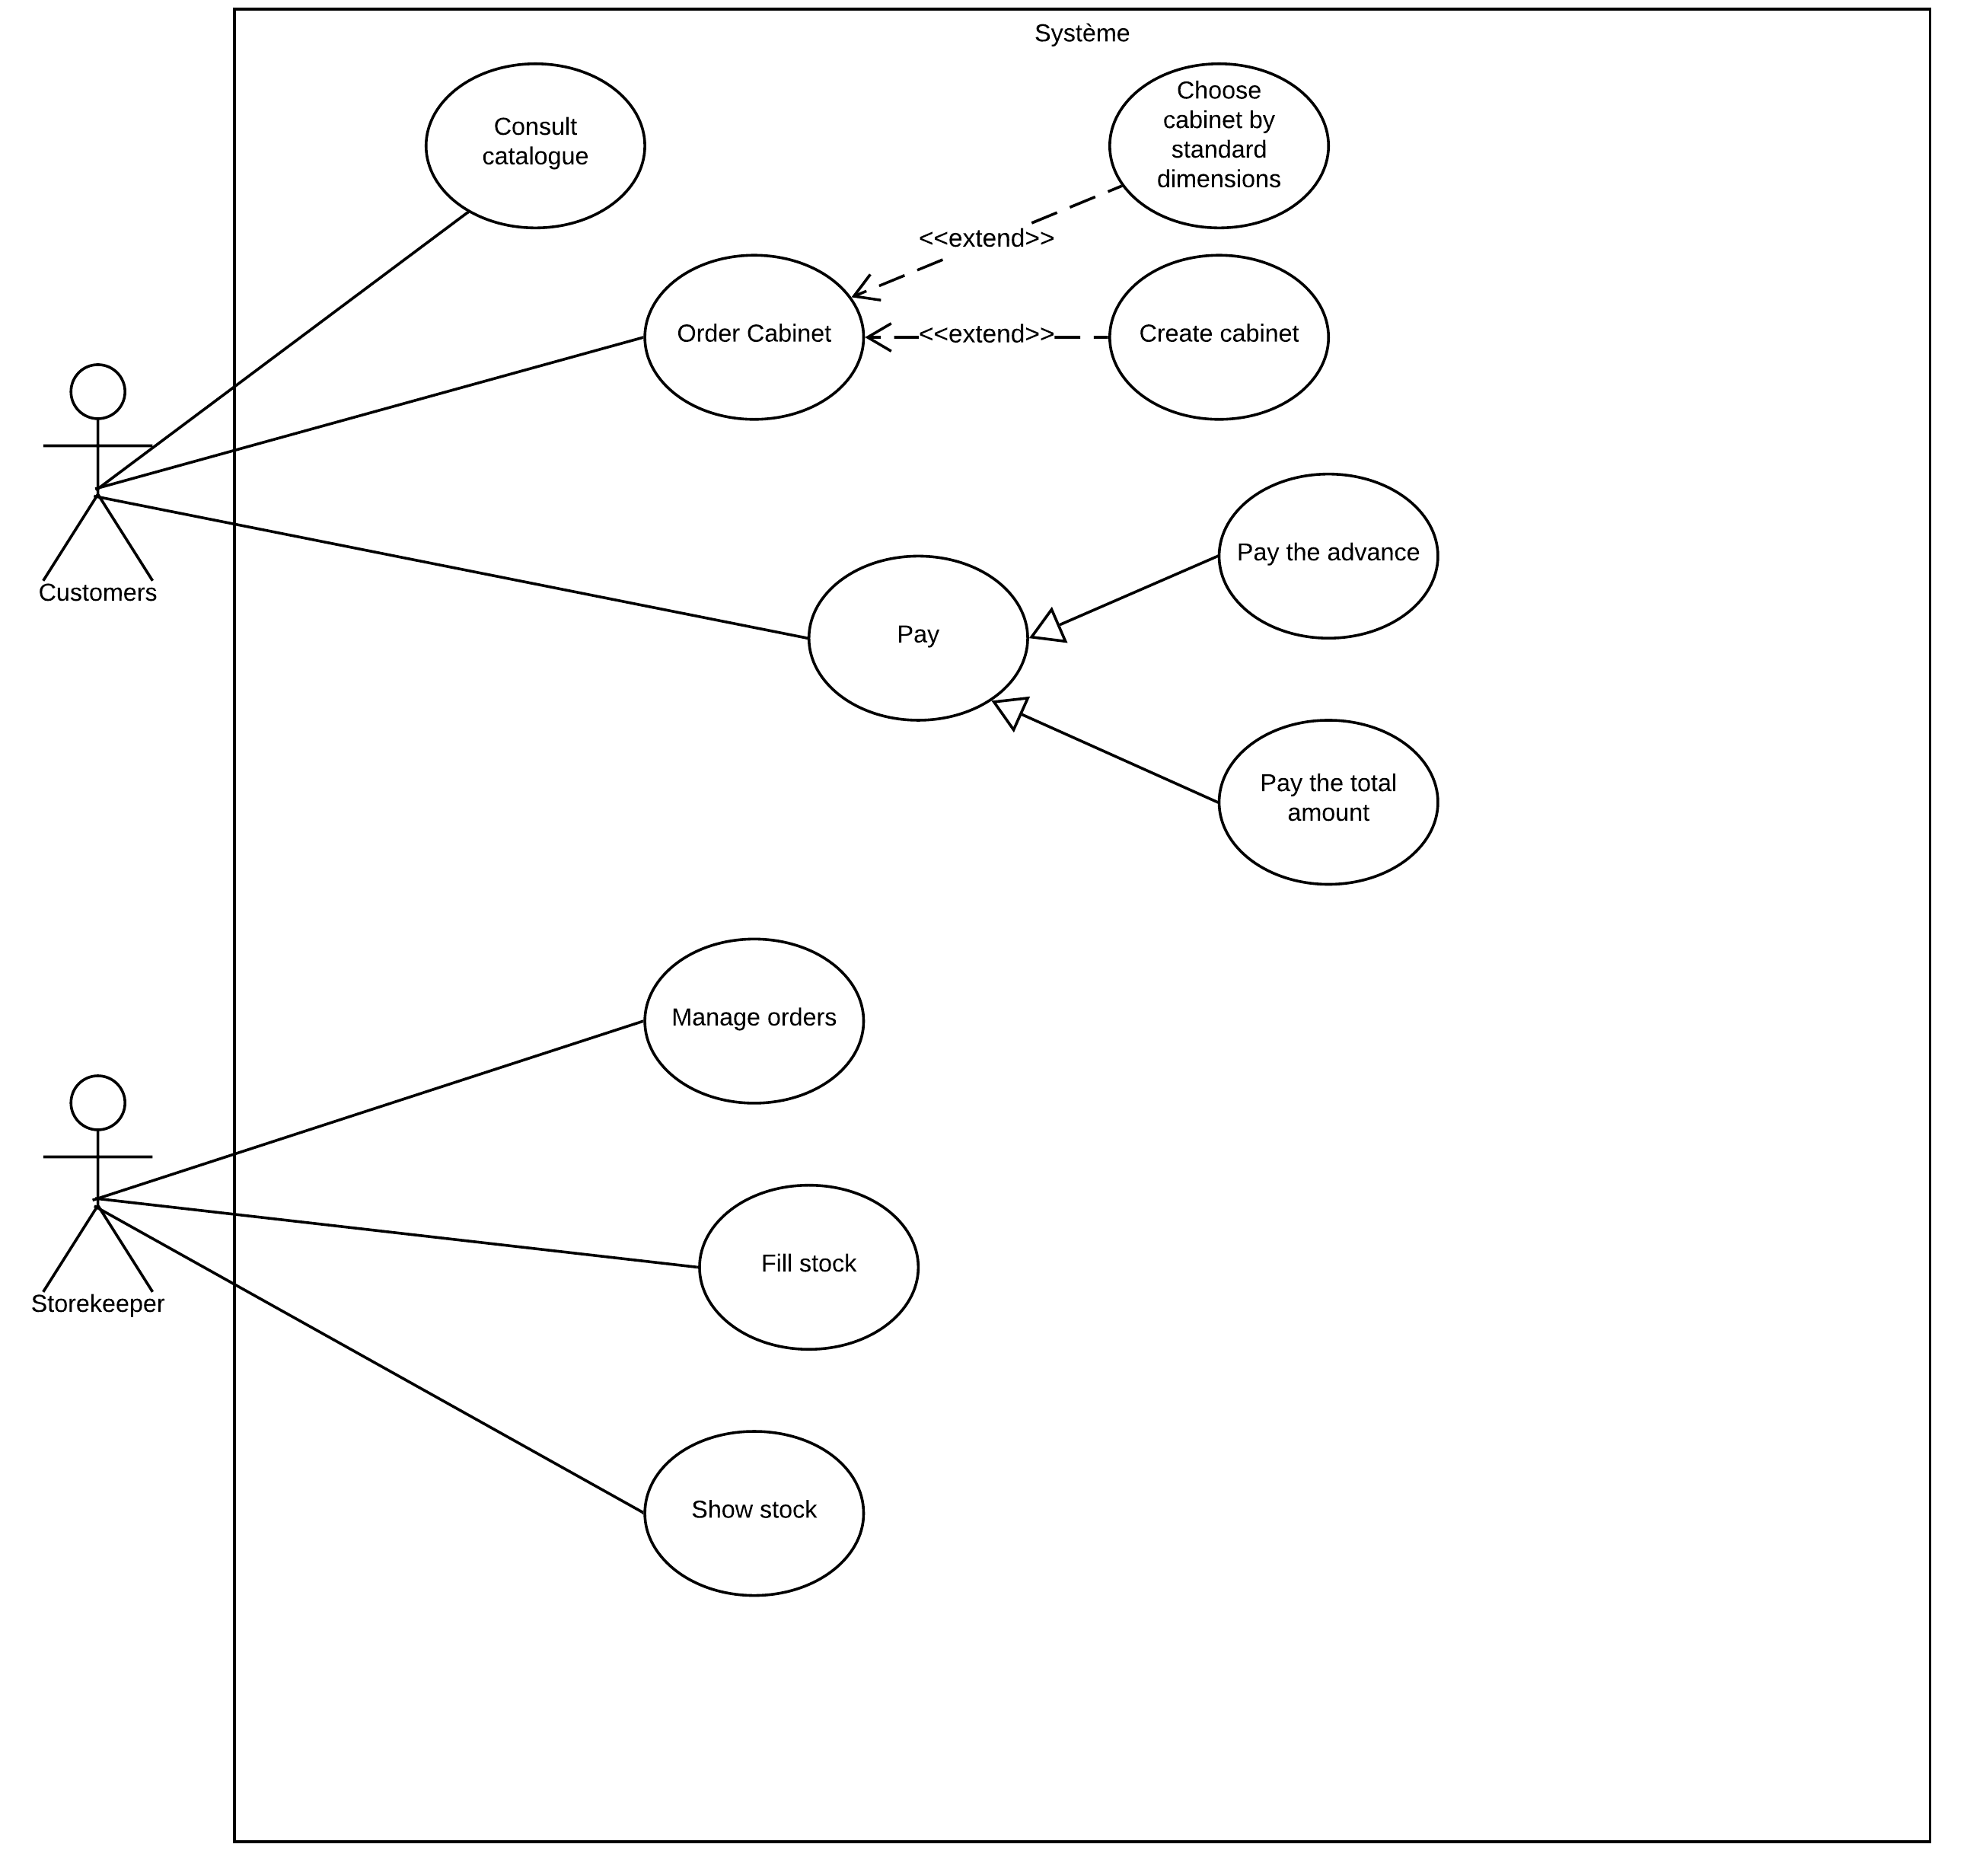
\includegraphics[width =\textwidth]{Figures/UseCaseDiagram.png}
			\rule{35em}{0.5pt}
			\caption{Use Case Diagram}
			\label{usecasediagram}
    	\end{figure*}
        \vfill
        
    \newpage
    \subsection{Class Diagram}
        \begin{figure*}[h!]
            \centering
			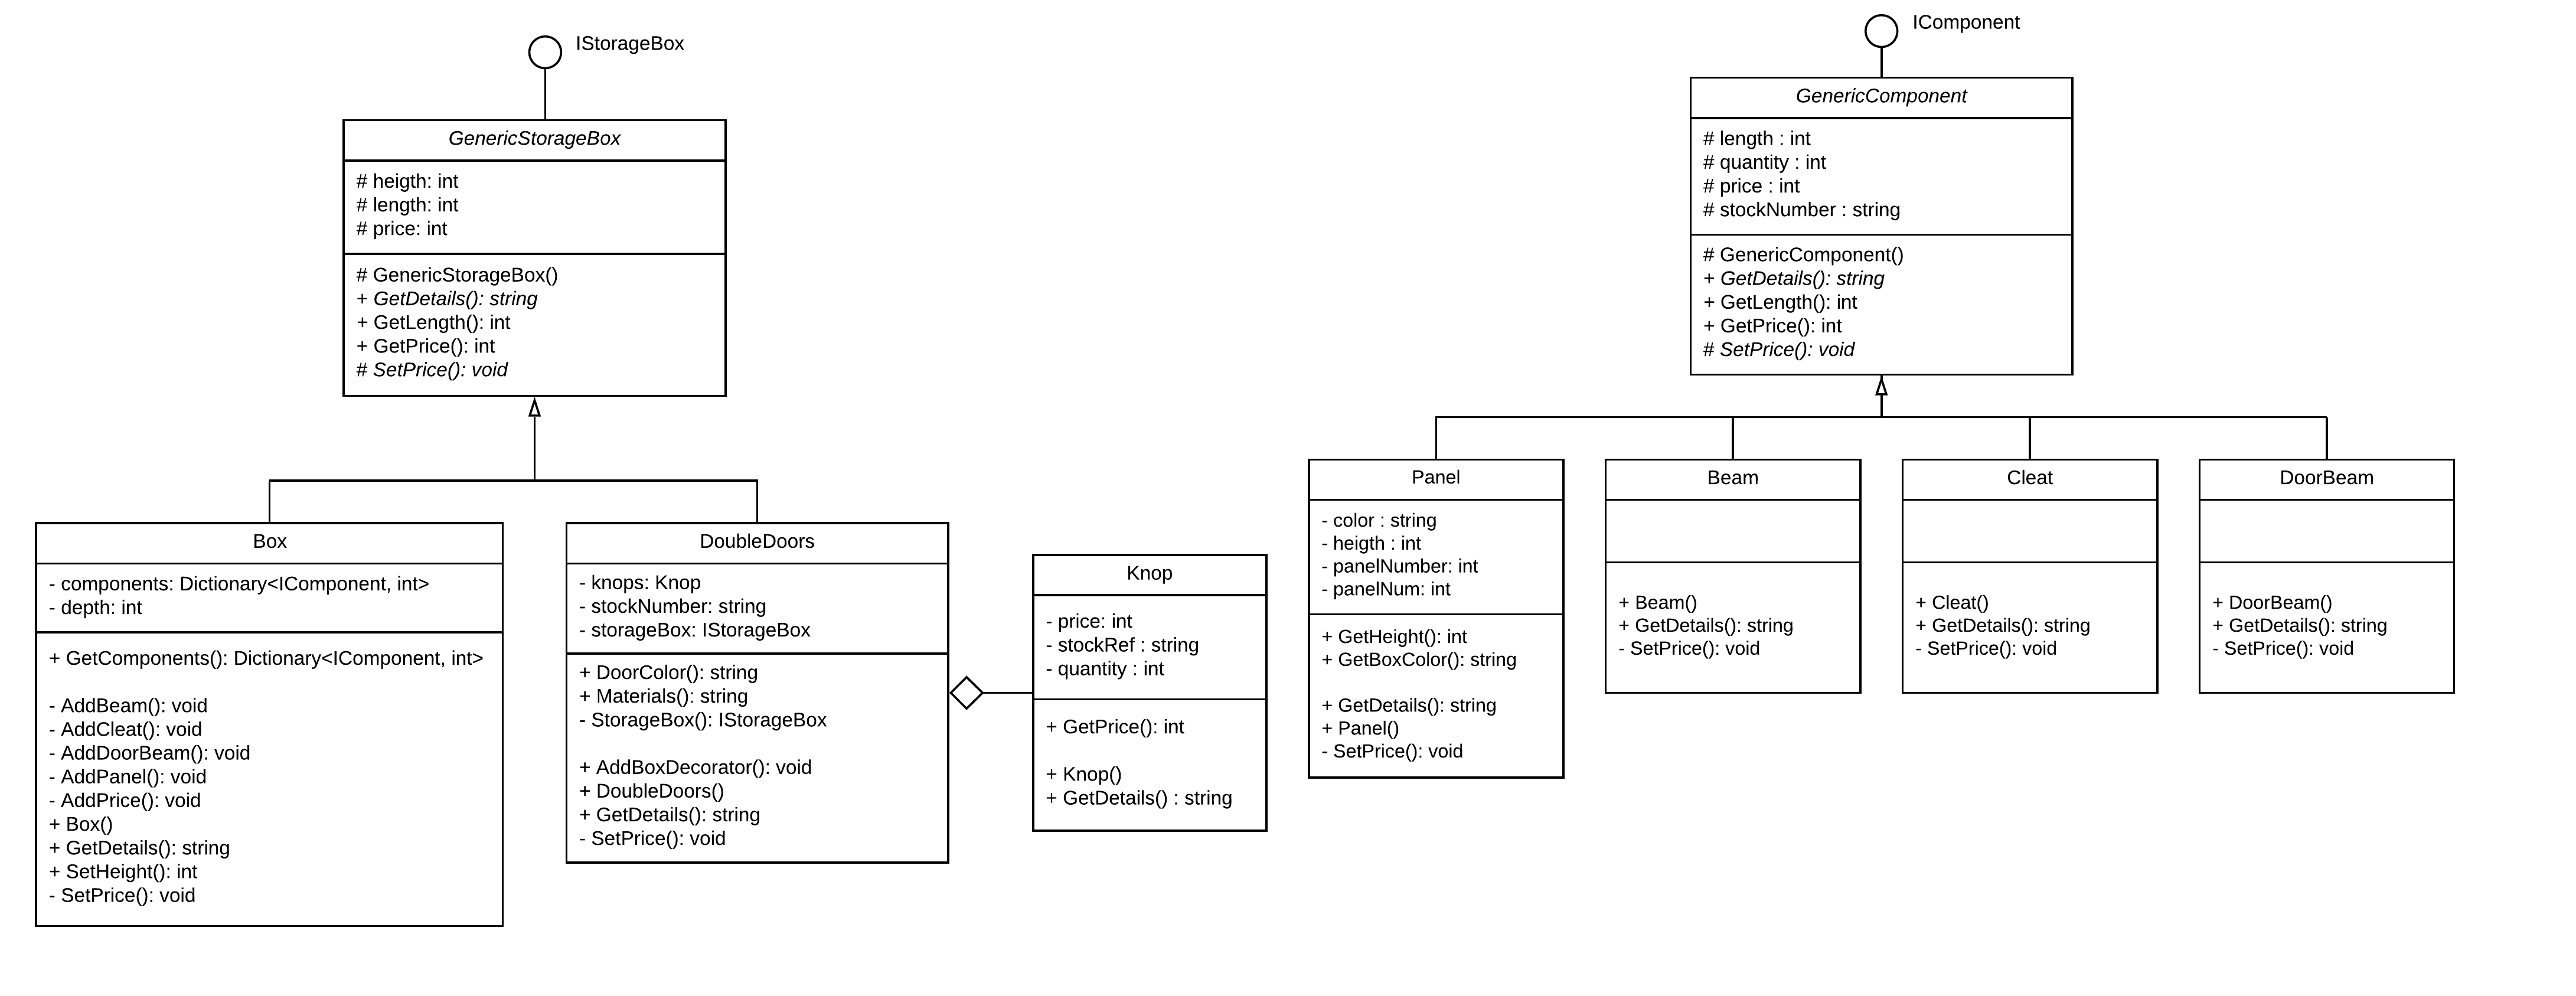
\includegraphics[width = 1.3\textwidth,angle = 90]{Figures/ClassDiagram-1.png}
			\rule{35em}{0.5pt}
			\caption{Class Diagram}
			\label{classdiagram}
    	\end{figure*}
    
    \newpage
    \subsection{Class Diagram – 2}
        \vfill
        \begin{figure*}[h!]
            \centering
			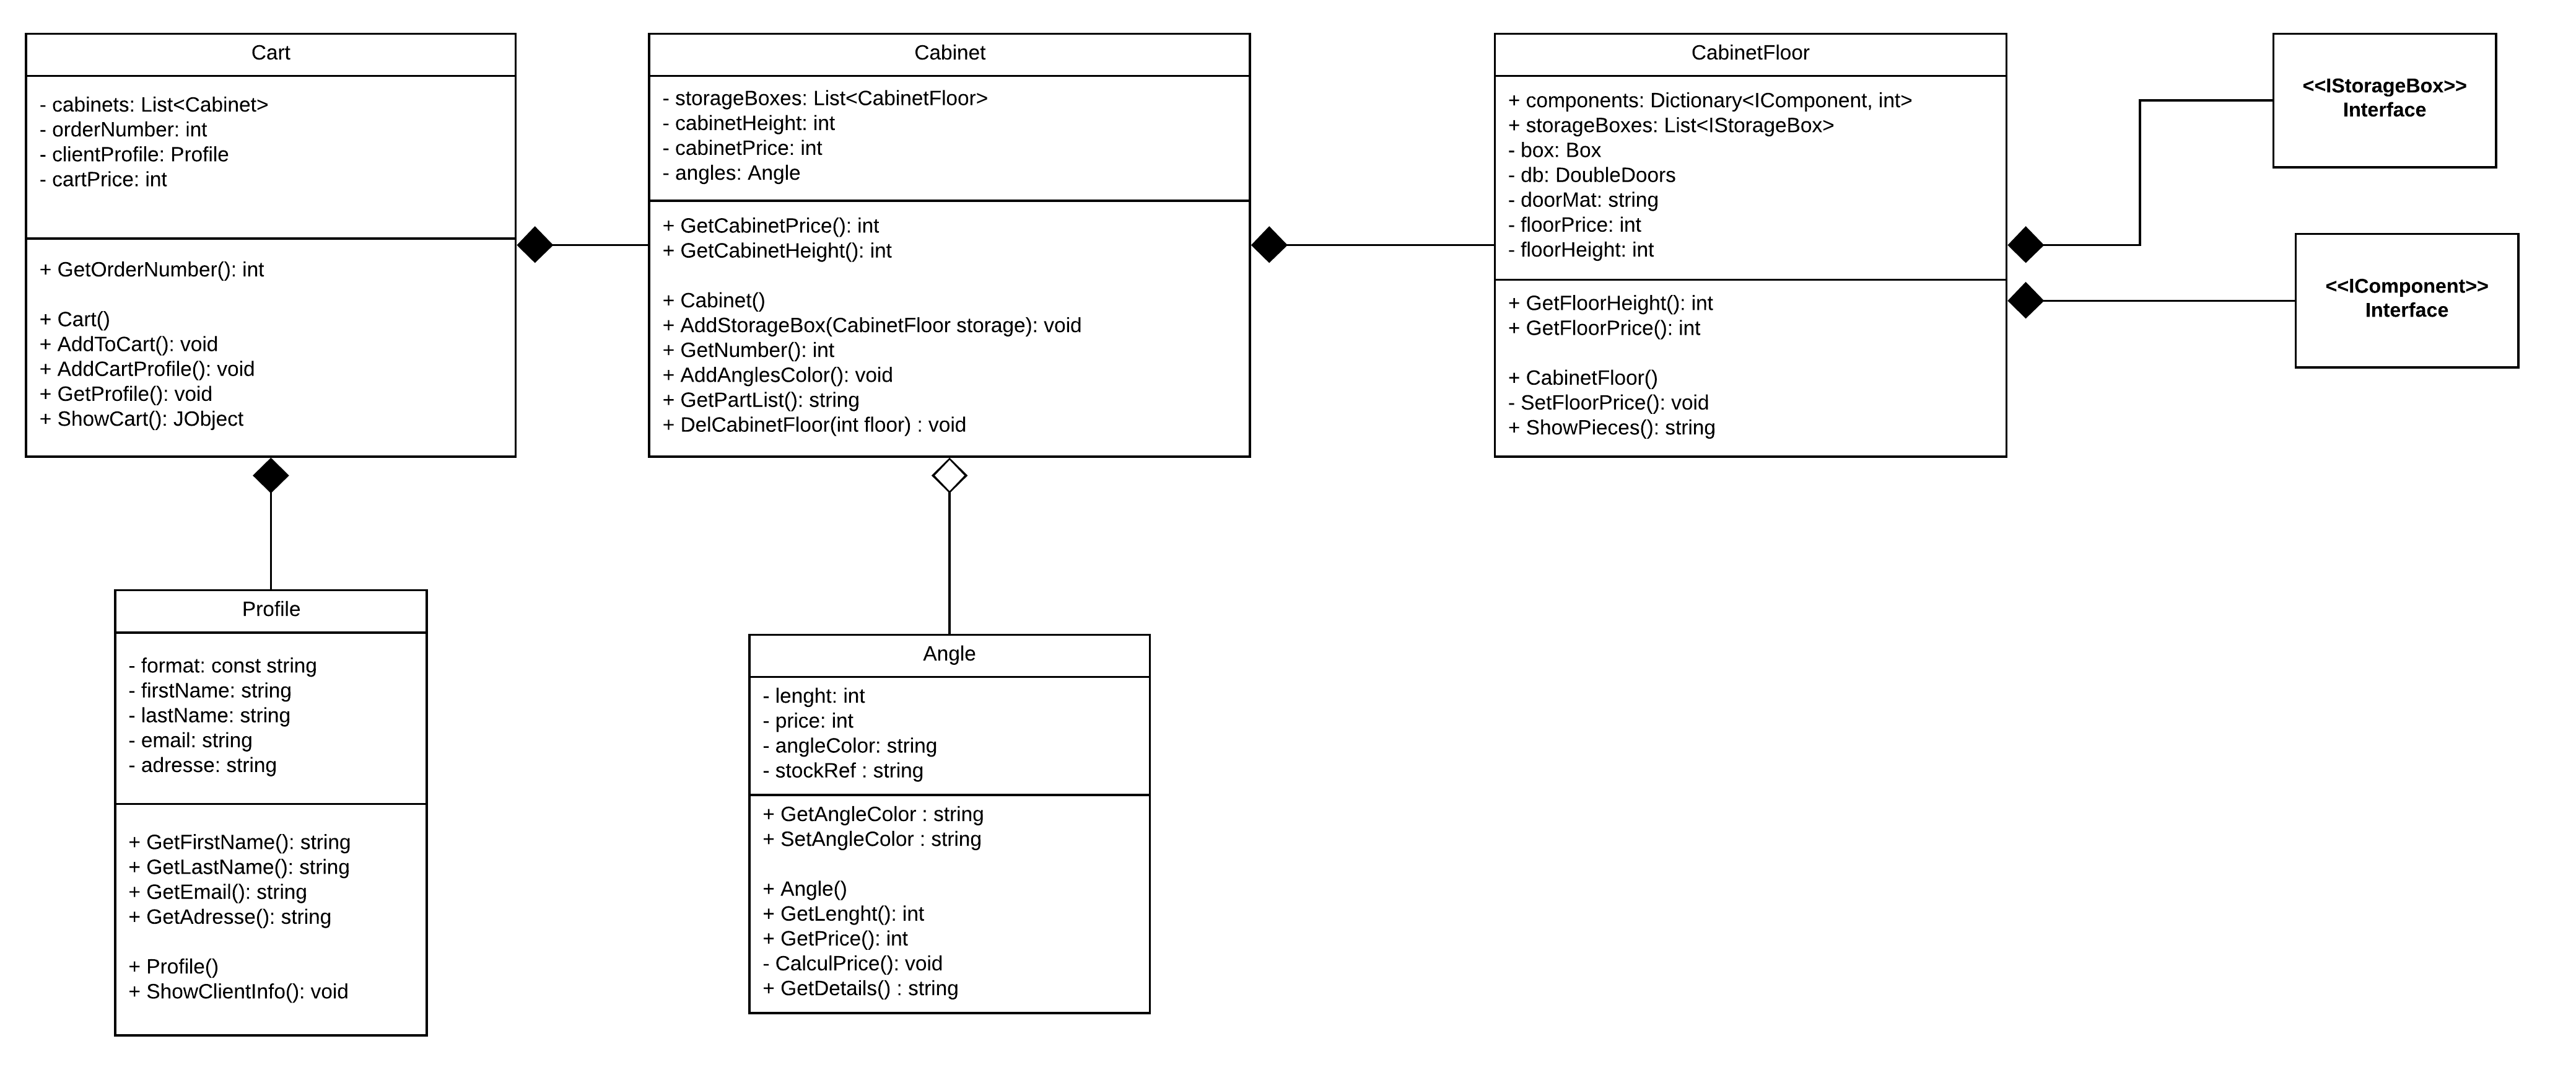
\includegraphics[width = 1.3\textwidth,angle = 90]{Figures/ClassDiagram-2.png}
			\rule{35em}{0.5pt}
			\caption{Class Diagram – 2}
			\label{classdiagram2}
    	\end{figure*}
        \vfill

\newpage
\section{User Interface}
\label{Userinterface}
    \subsection{Homepage}
        \vfill
        \begin{figure*}[h!]
            \centering
    		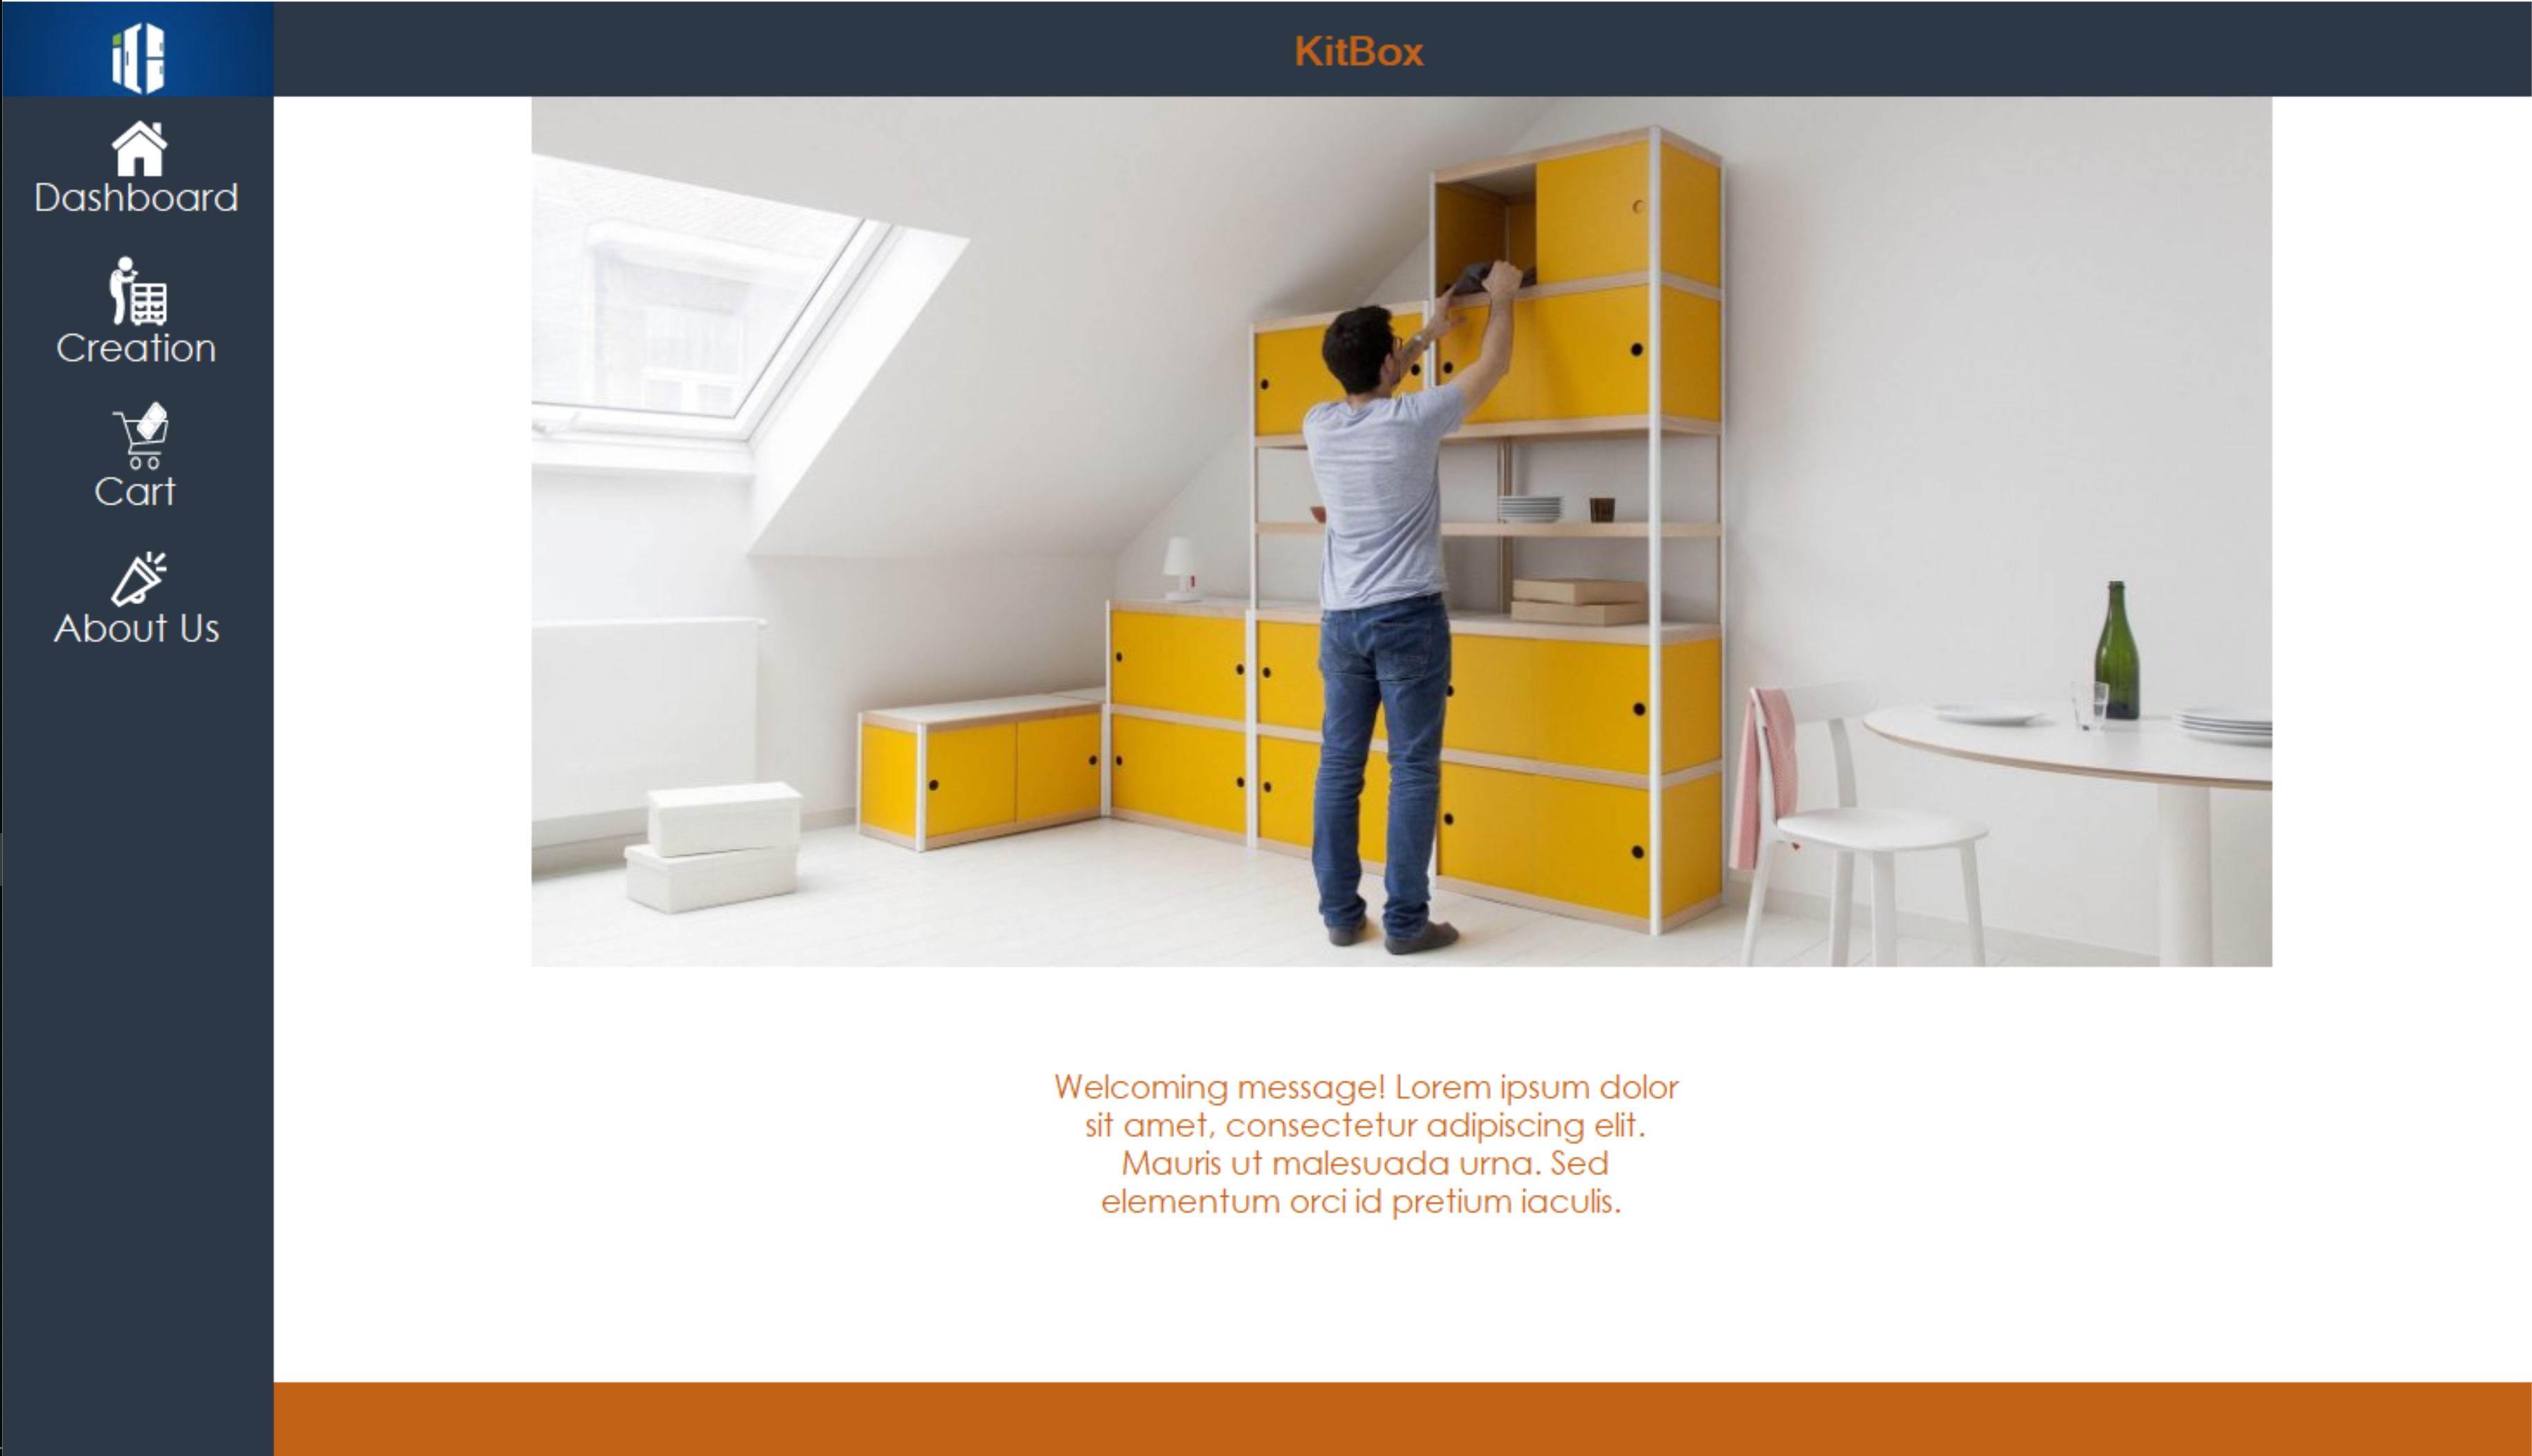
\includegraphics[width =1.2\textwidth,angle = 90]{Figures/Homepage.PNG}
    		\rule{35em}{0.5pt}
    		\caption{Home welcoming page}
    		\label{homepage}
    	\end{figure*}
    	\vfill
    	
	\newpage
	\subsection{Creation welcoming page}
    	\vfill
        \begin{figure*}[h!]
            \centering
    		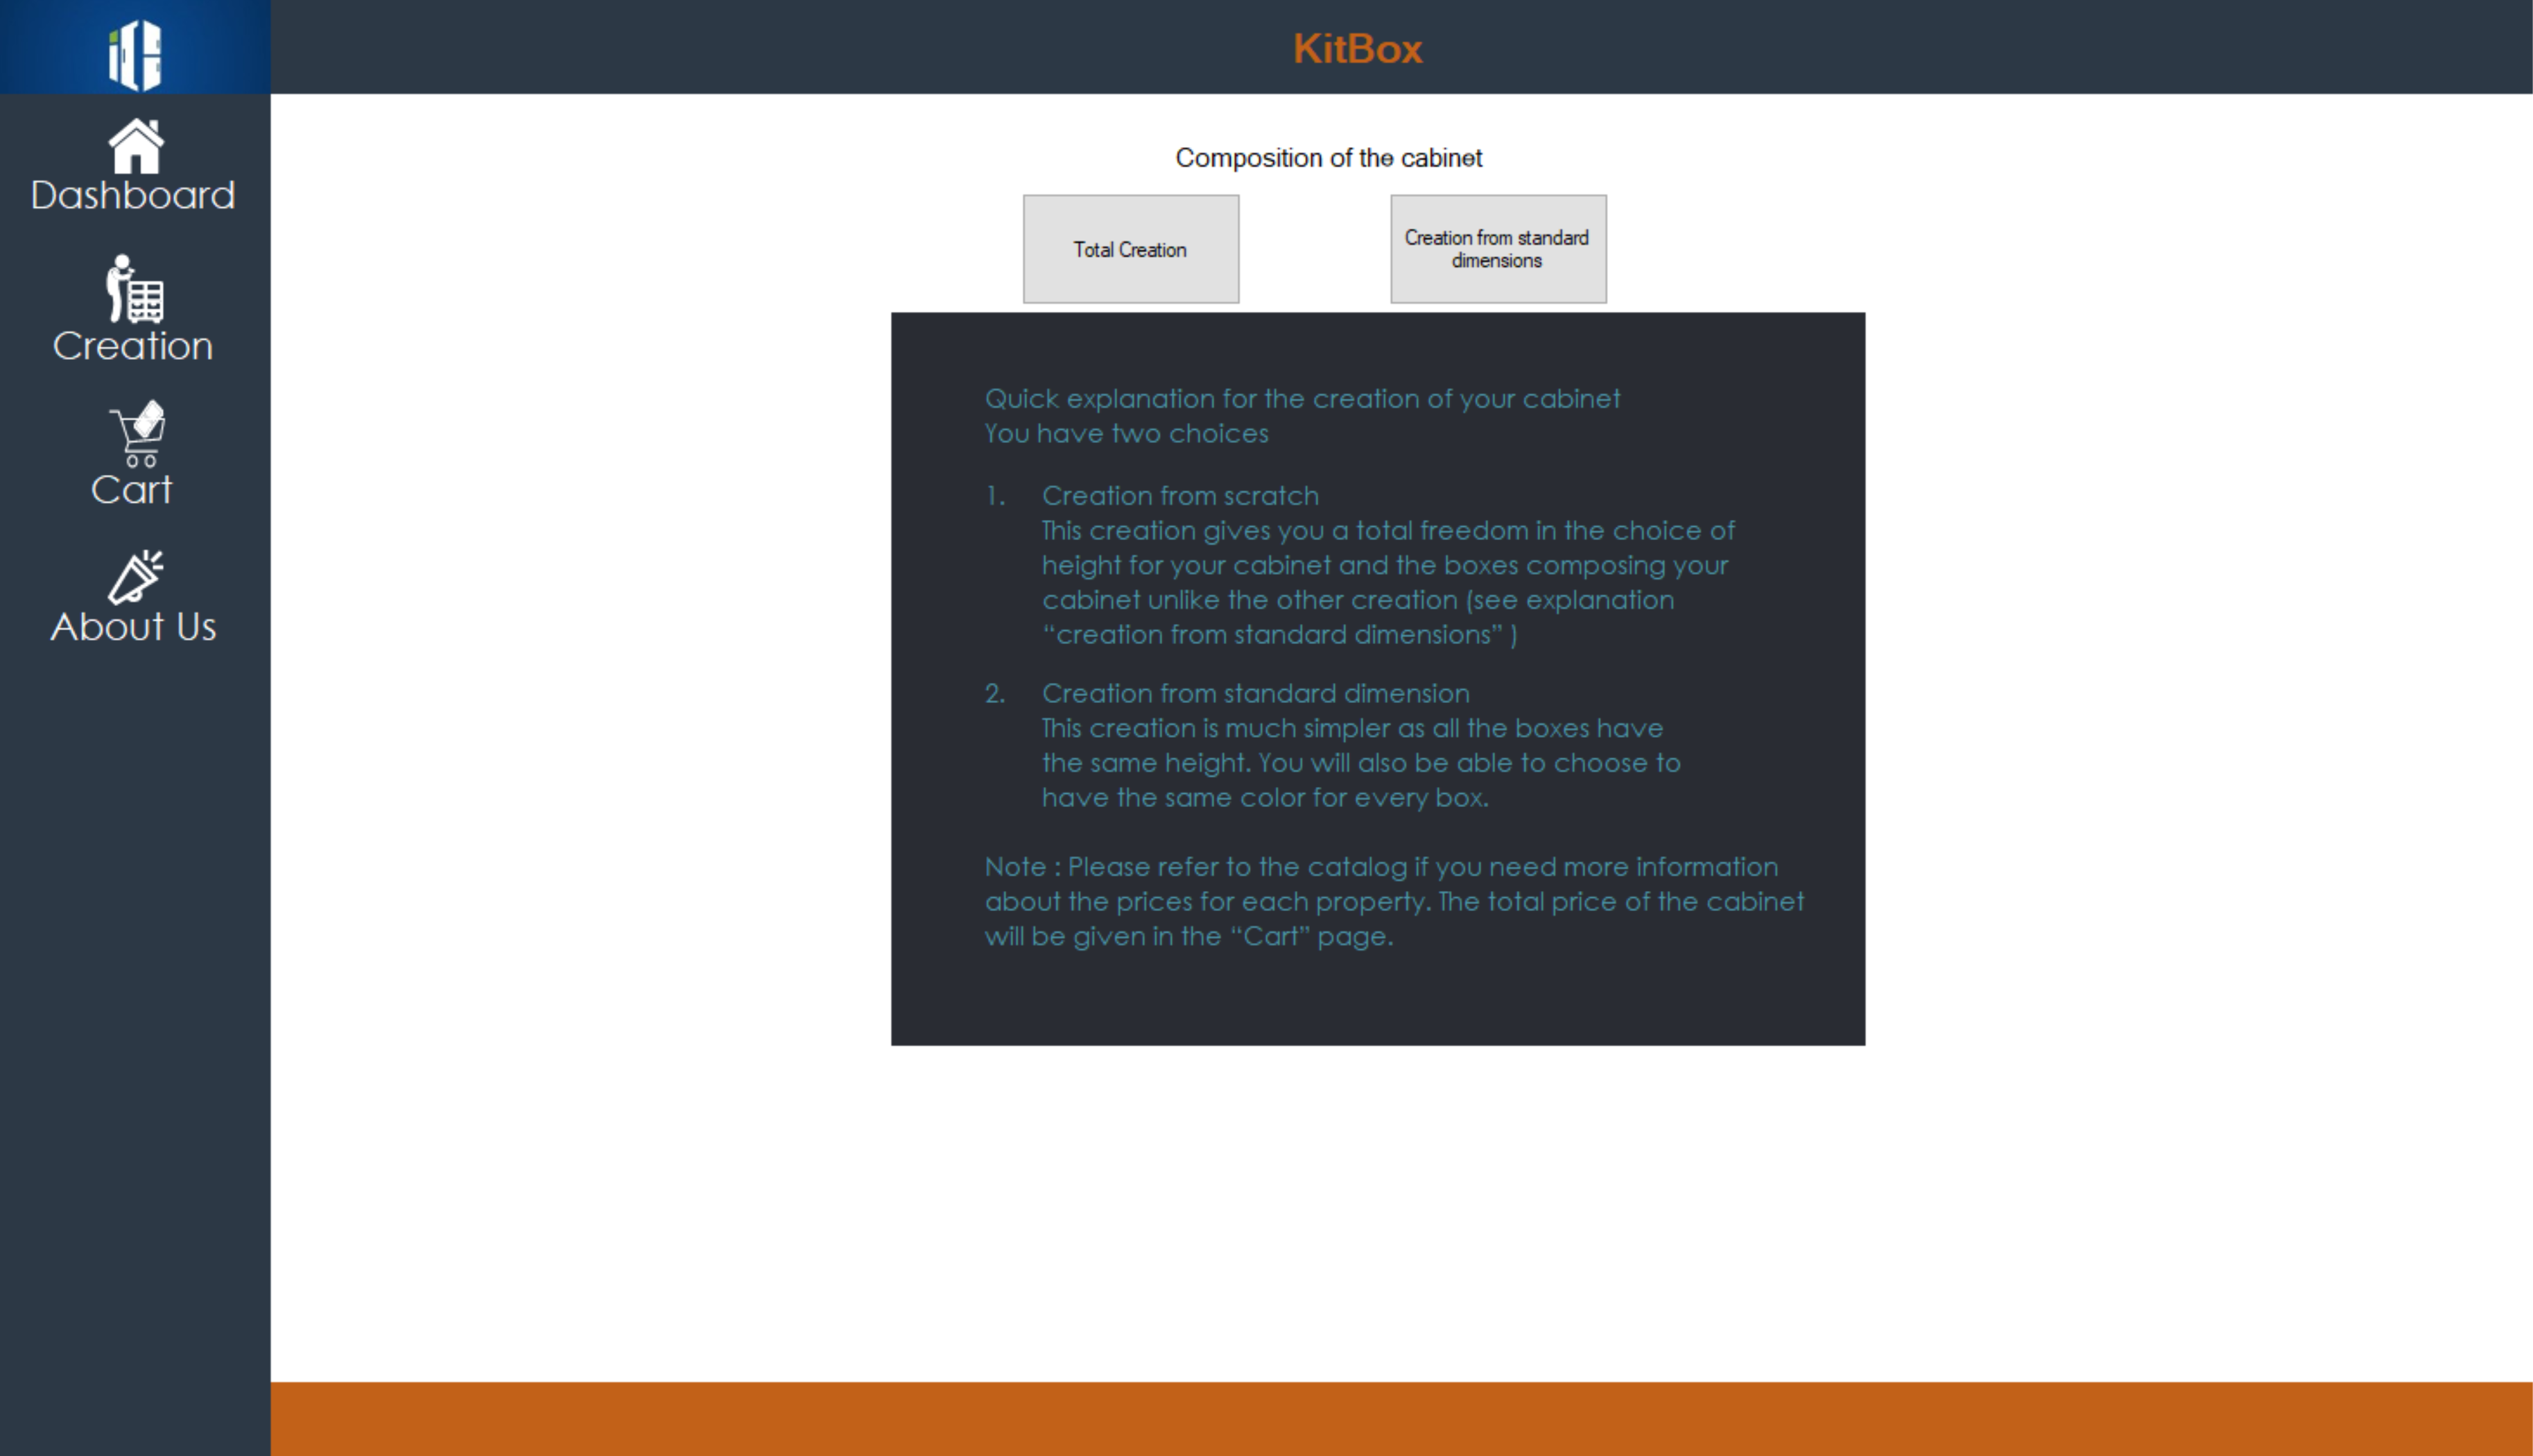
\includegraphics[width =1.2\textwidth,angle = 90]{Figures/creationWelcome.PNG}
    		\rule{35em}{0.5pt}
    		\caption{Creation welcoming page explaining the choices of creation}
    		\label{welcomtab}
    	\end{figure*}
    	\vfill
    	
	\newpage
	\subsection{Creation from Scratch}
    	\vfill
        \begin{figure*}[h!]
            \centering
    		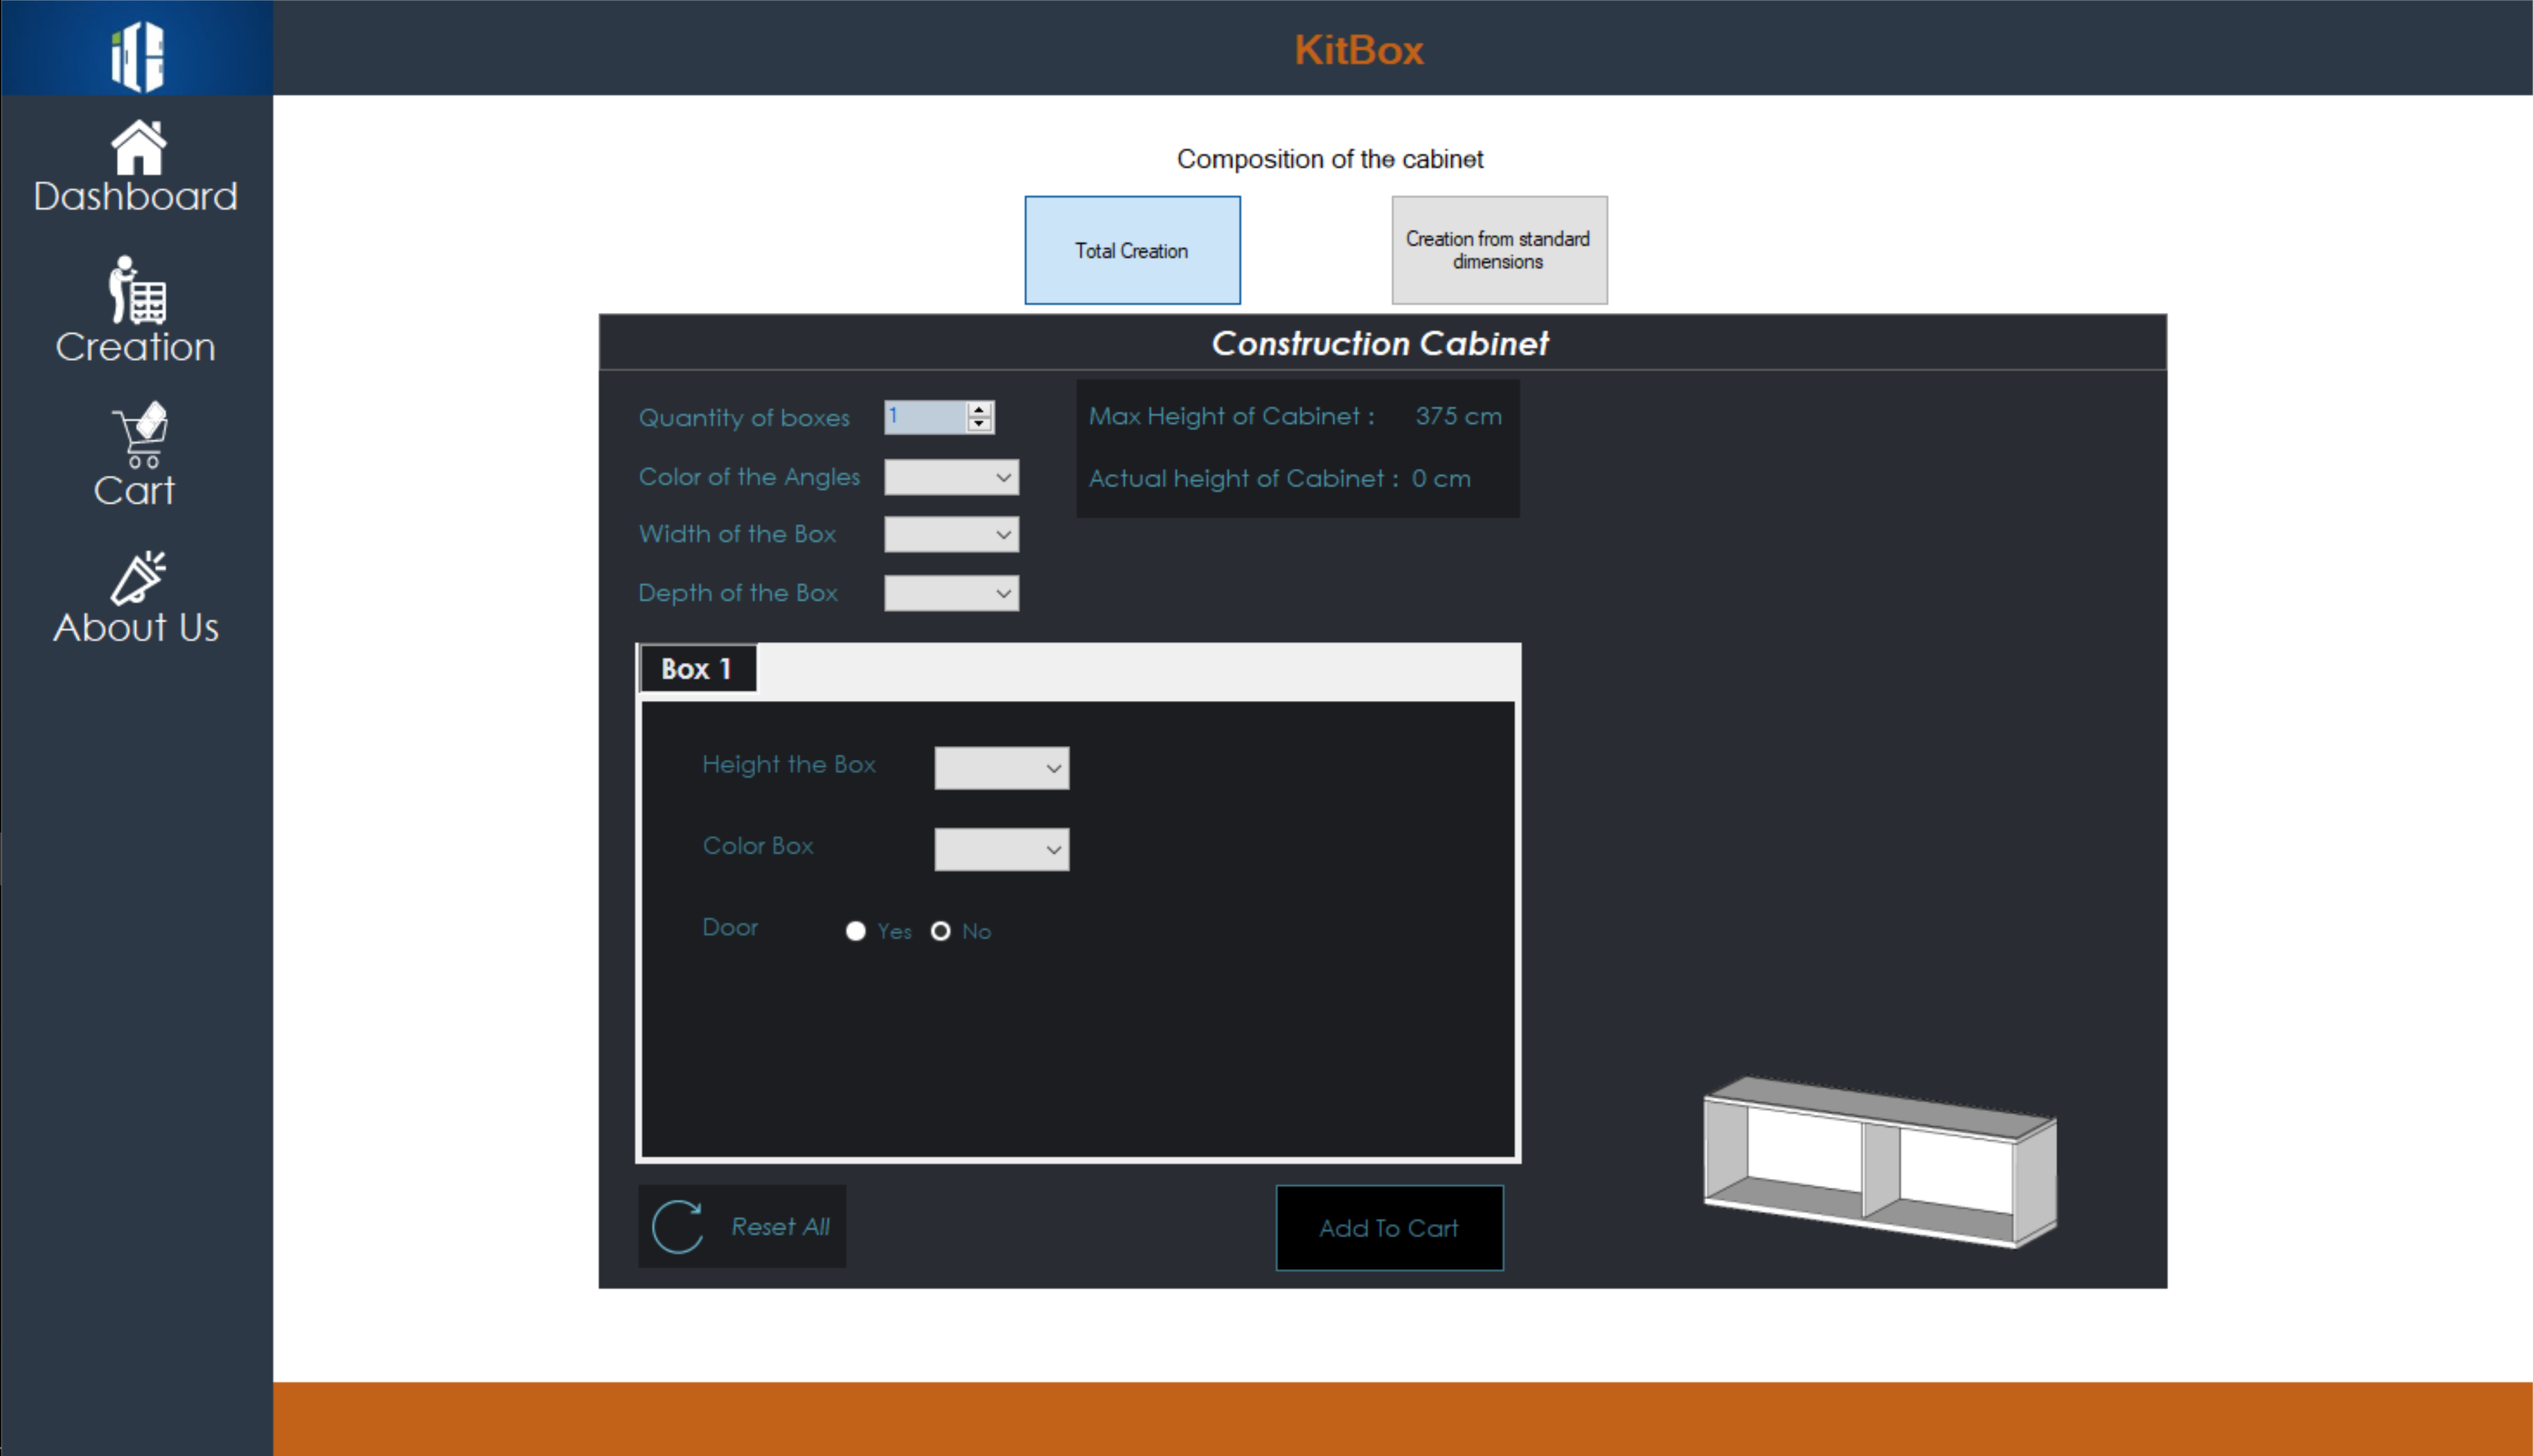
\includegraphics[width =1.2\textwidth,angle = 90]{Figures/CreationScratch.PNG}
    		\rule{35em}{0.5pt}
    		\caption{Creation from Scratch initial state}
    		\label{ordertab}
    	\end{figure*}
    	\vfill
    	
	\newpage
	\subsection{Creation from Scratch filled}
    	\vfill
        \begin{figure*}[h!]
            \centering
    		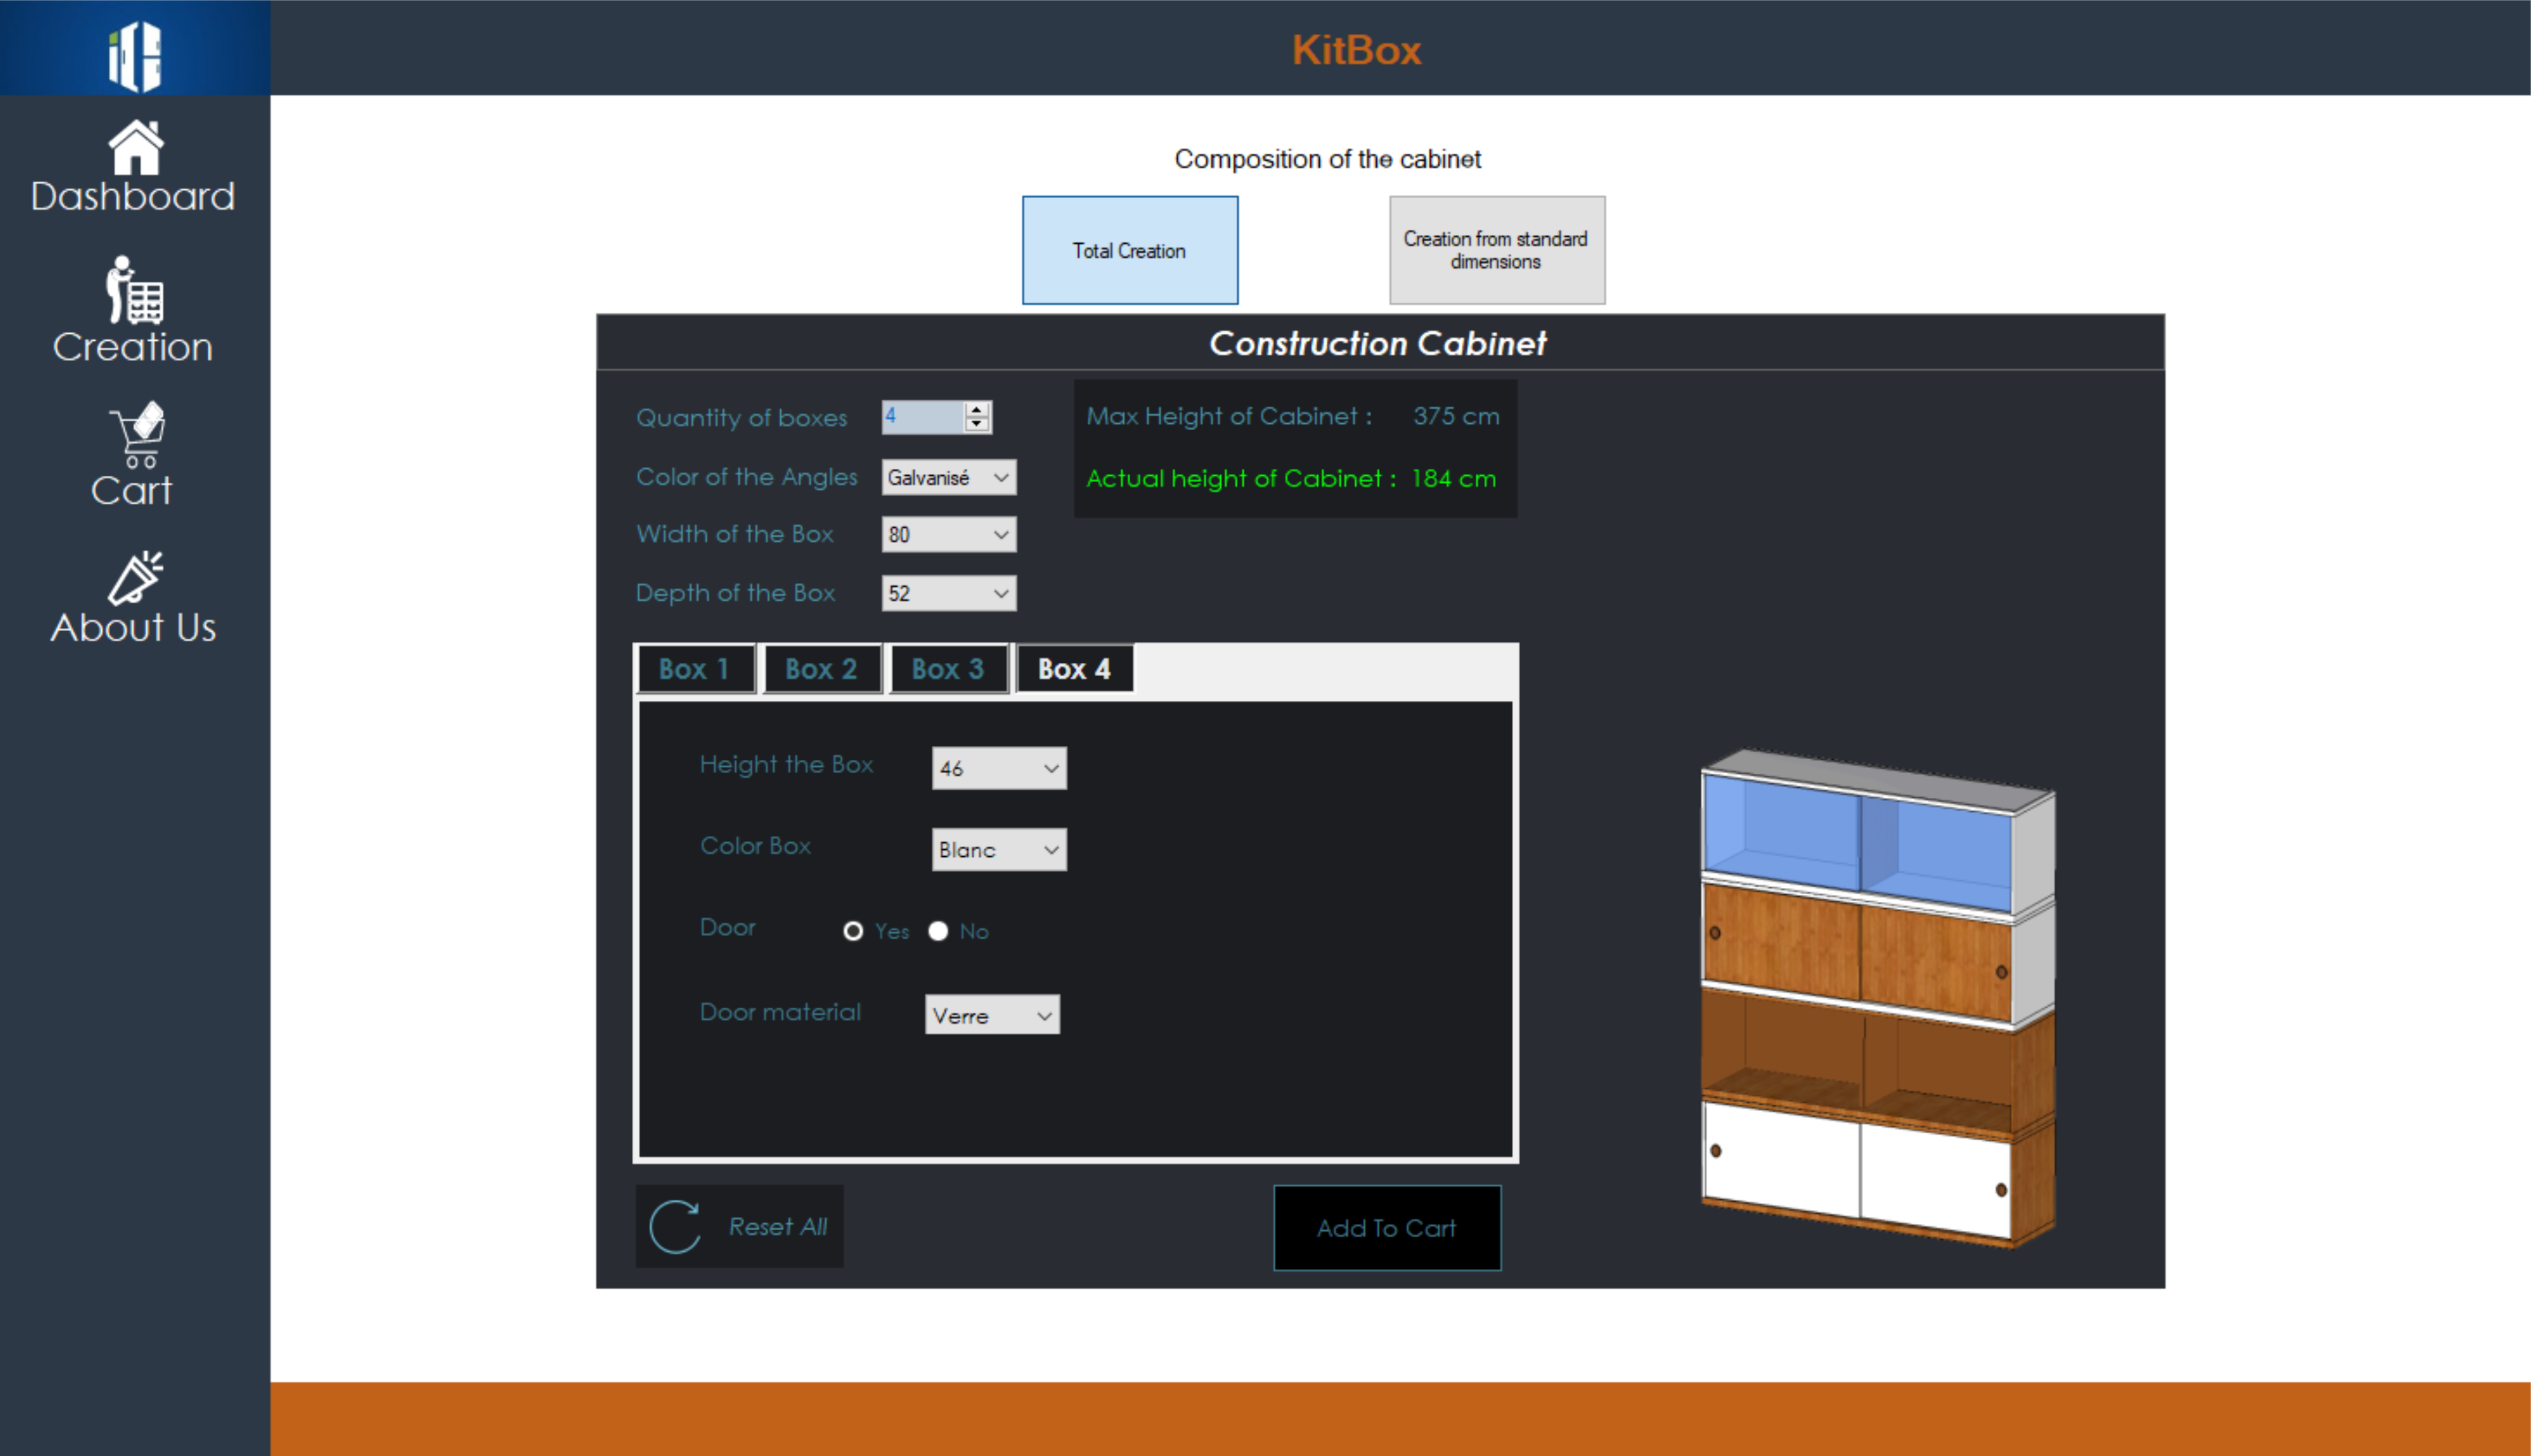
\includegraphics[width =1.2\textwidth,angle = 90]{Figures/CreationScratchFilled.PNG}
    		\rule{35em}{0.5pt}
    		\caption{Creation from Scratch after filling all the features}
    		\label{scratchtab}
    	\end{figure*}
    	\vfill
    	
	\newpage
	\subsection{Creation from standard dimensions}
    	\vfill
        \begin{figure*}[h!]
            \centering
    		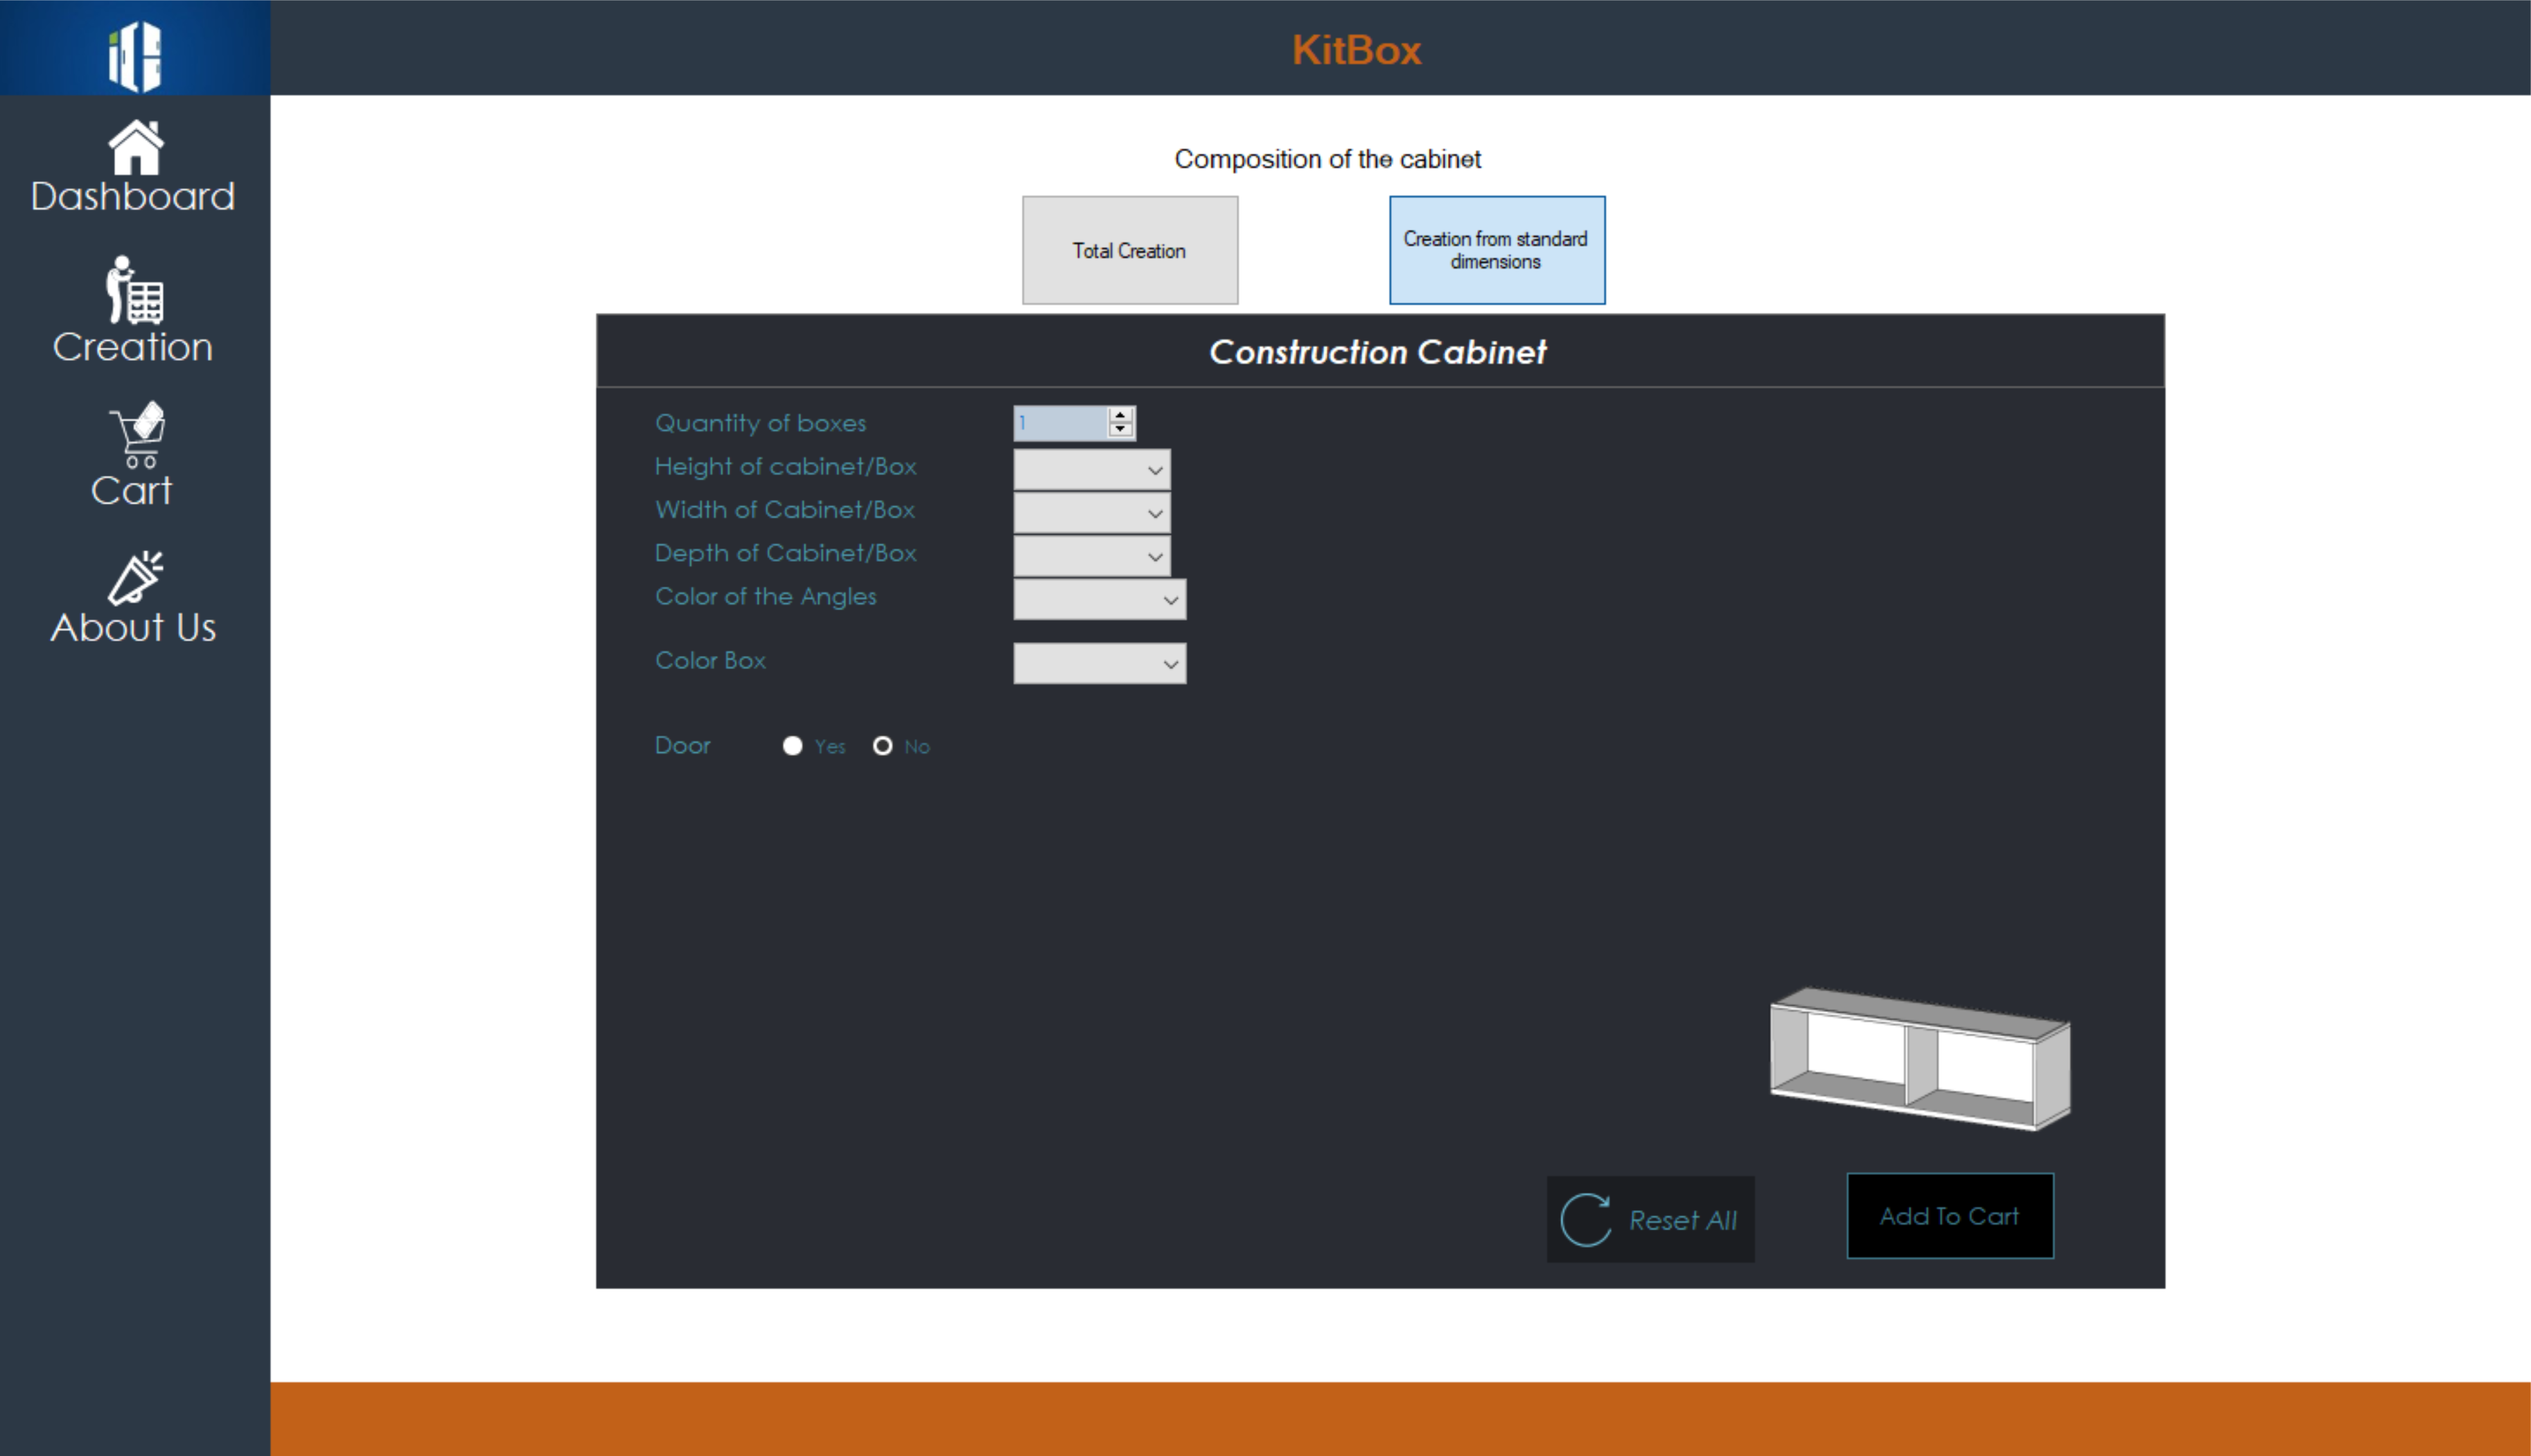
\includegraphics[height=110truemm,angle = 90]{Figures/CreationStandard.PNG}
    		\rule{35em}{0.5pt}
    		\caption{Creation from standard dimensions initial state}
    		\label{standardtab}
    	\end{figure*}
    	\vfill
    	
	\newpage
	\subsection{Creation from standard dimensions filled}
    	\vfill
        \begin{figure*}[h!]
            \centering
    		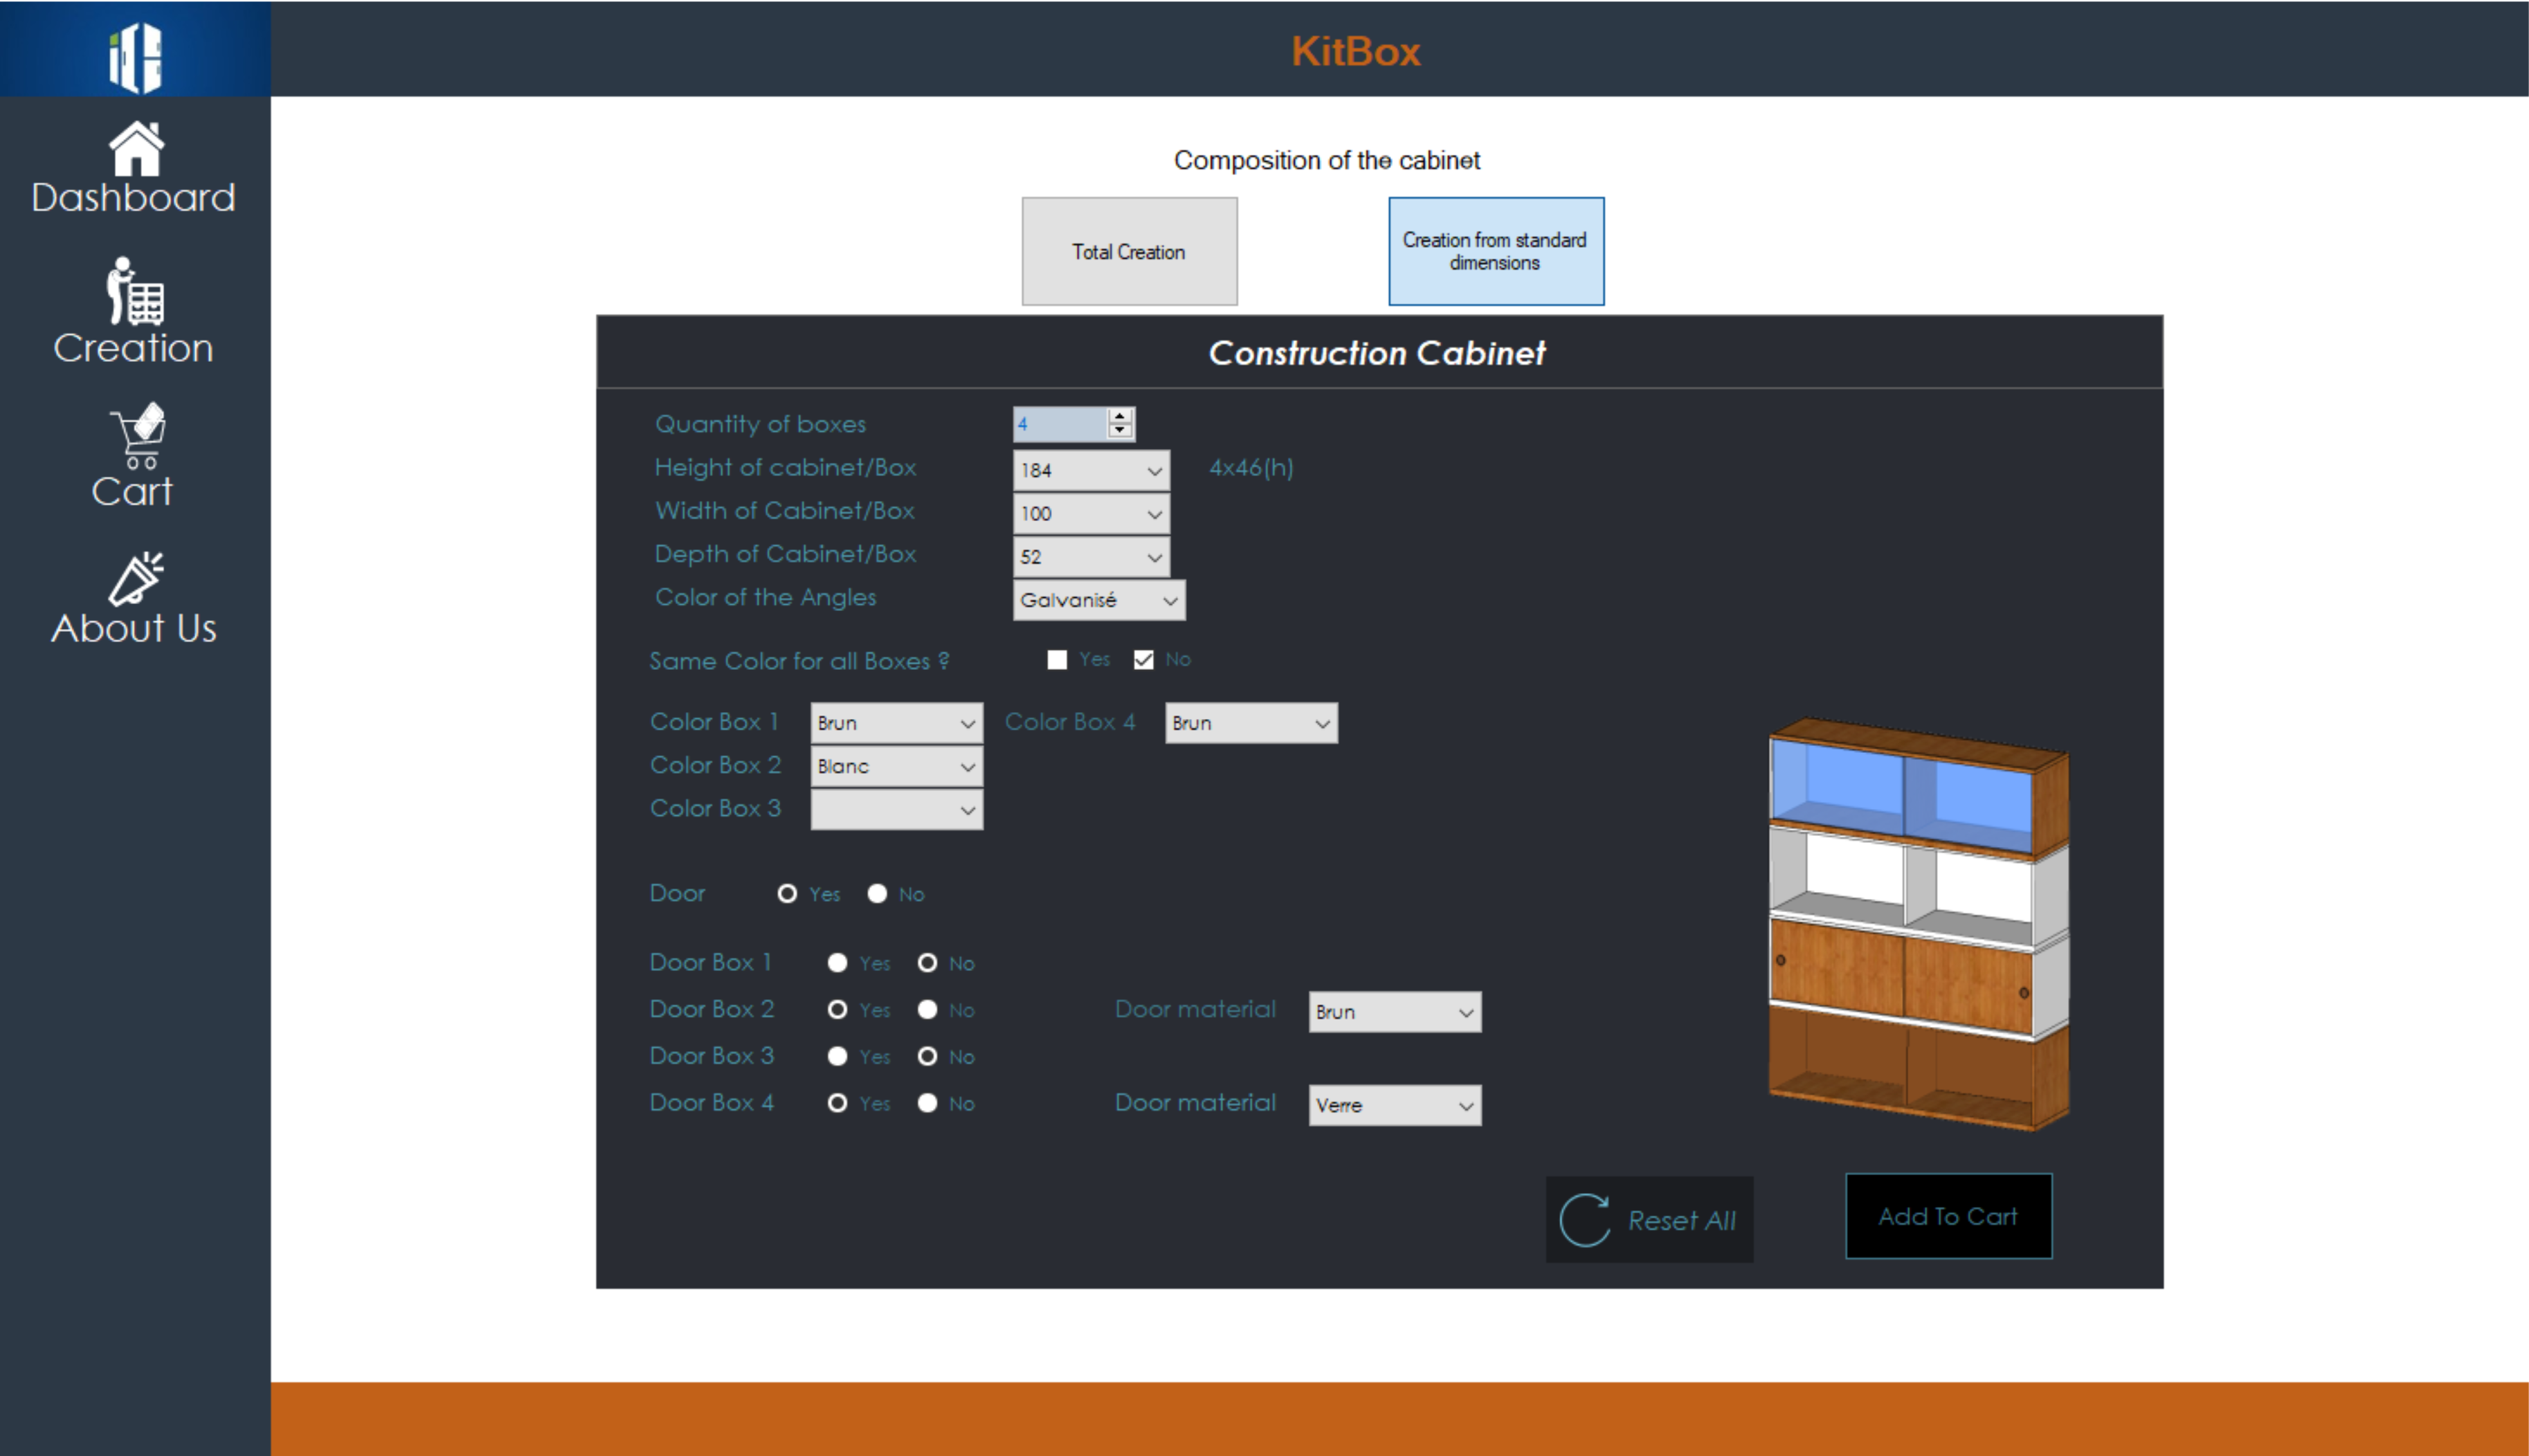
\includegraphics[height=110truemm,angle = 90]{Figures/CreationStandardFilled.PNG}
    		\rule{35em}{0.5pt}
    		\caption{Creation from standard dimensions after filling all features}
    		\label{standardtabfilled}
    	\end{figure*}
    	\vfill
	
	\newpage
	\subsection{Cart page}
    	\vfill
        \begin{figure*}[h!]
            \centering
    		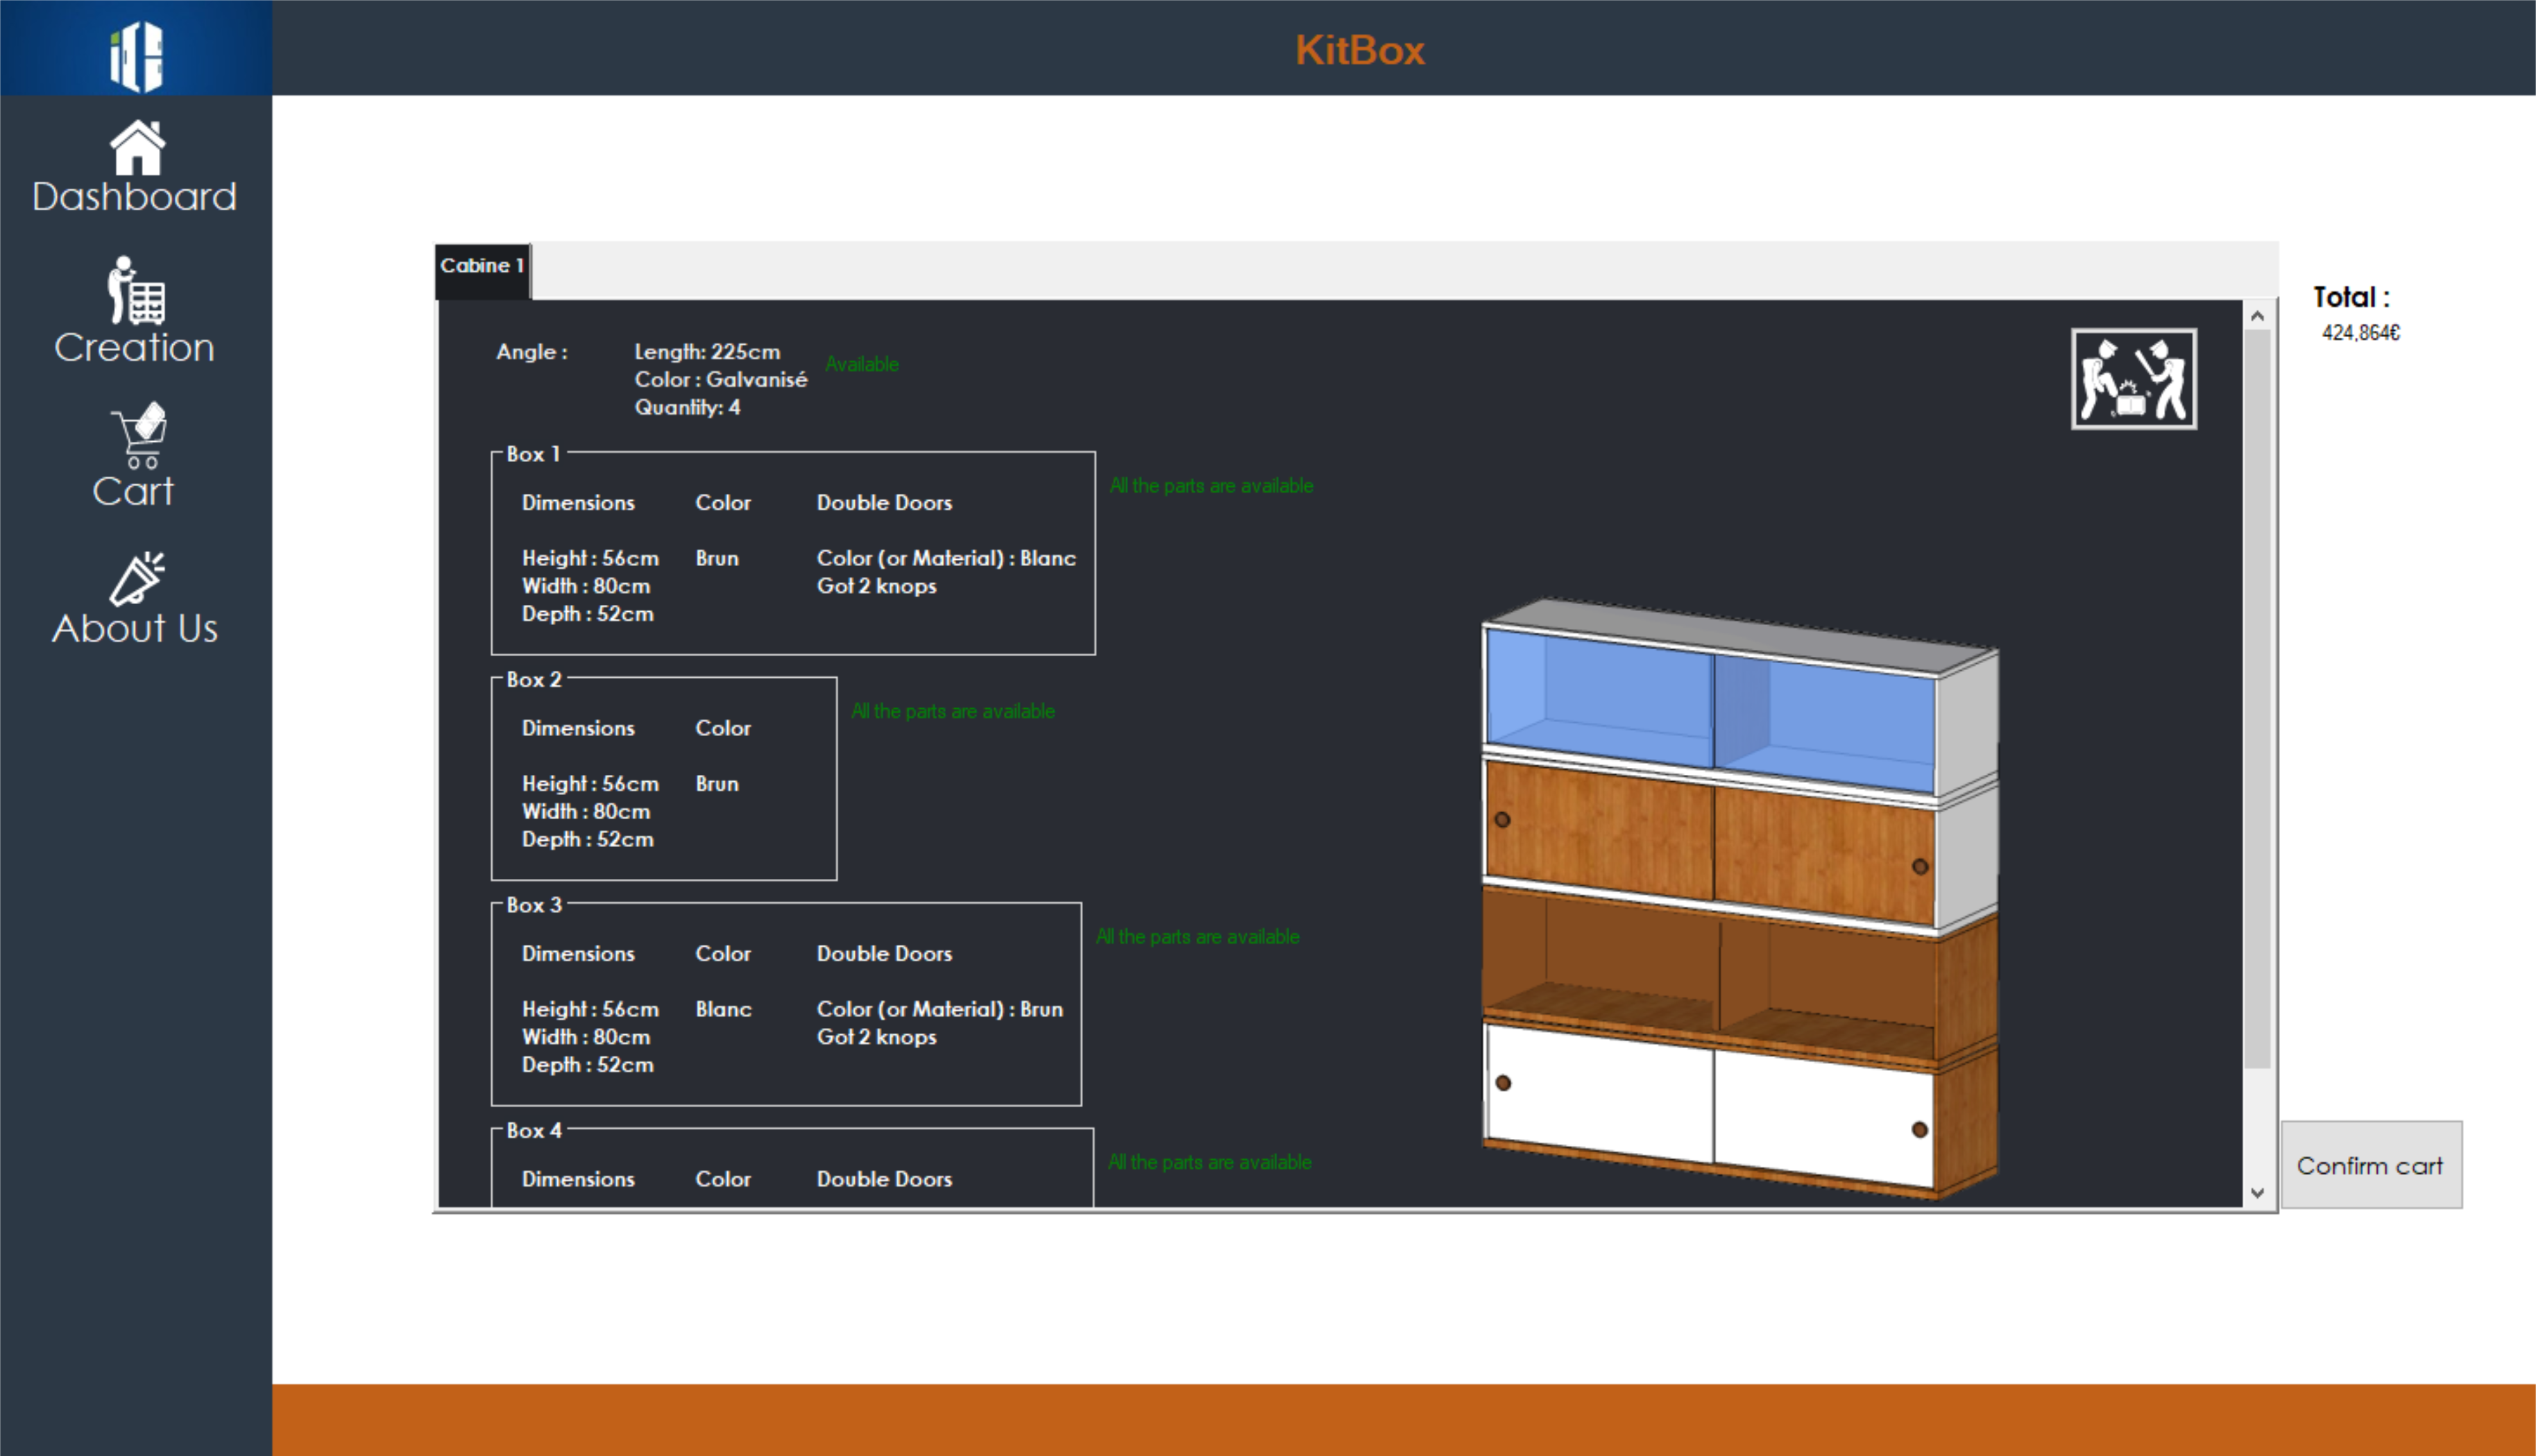
\includegraphics[width =1.2\textwidth,angle = 90]{Figures/CartPage.PNG}
    		\rule{35em}{0.5pt}
    		\caption{Cart page containing one four floors cabinet}
    		\label{carttab}
    	\end{figure*}
    	\vfill
    	
    \newpage
	\subsection{Cart page with mail}
    	\vfill
        \begin{figure*}[h!]
            \centering
    		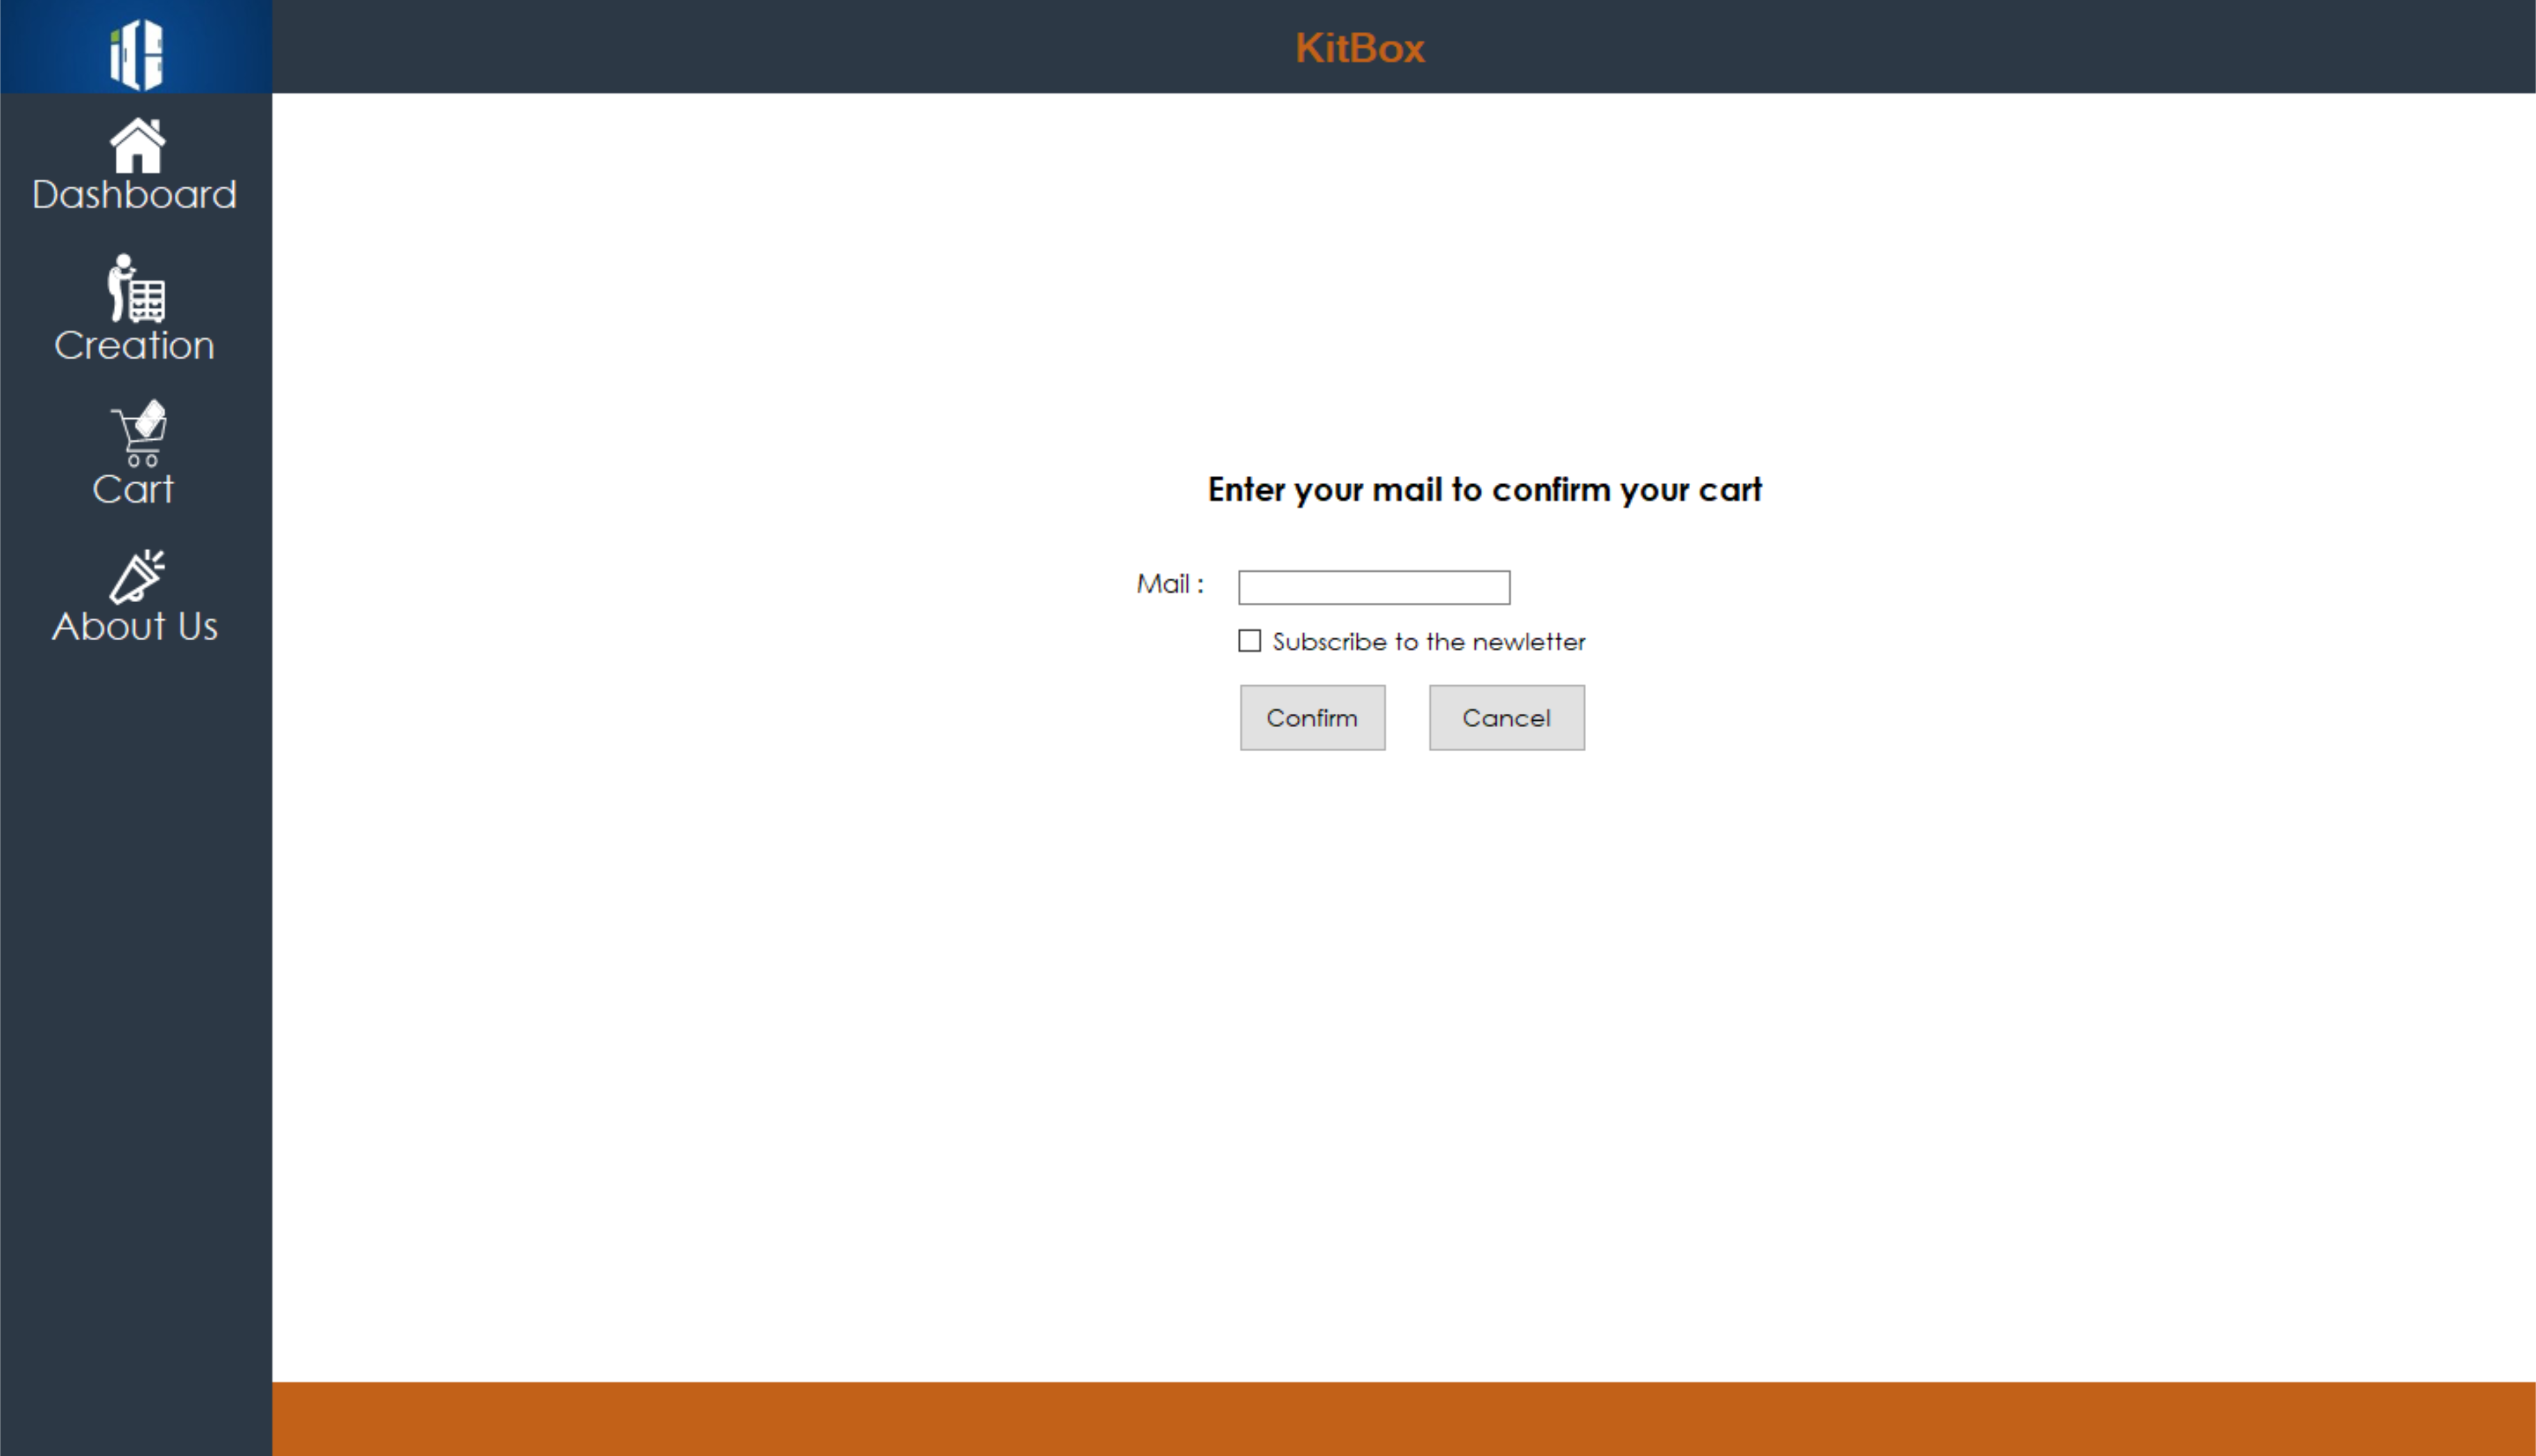
\includegraphics[width =1.2\textwidth,angle = 90]{Figures/CartPageMail.PNG}
    		\rule{35em}{0.5pt}
    		\caption{Client credentials to order cabinet}
    		\label{authtab}
    	\end{figure*}
    	\vfill
    	
    \newpage
	\subsection{About Us page}
    	\vfill
        \begin{figure*}[h!]
            \centering
    		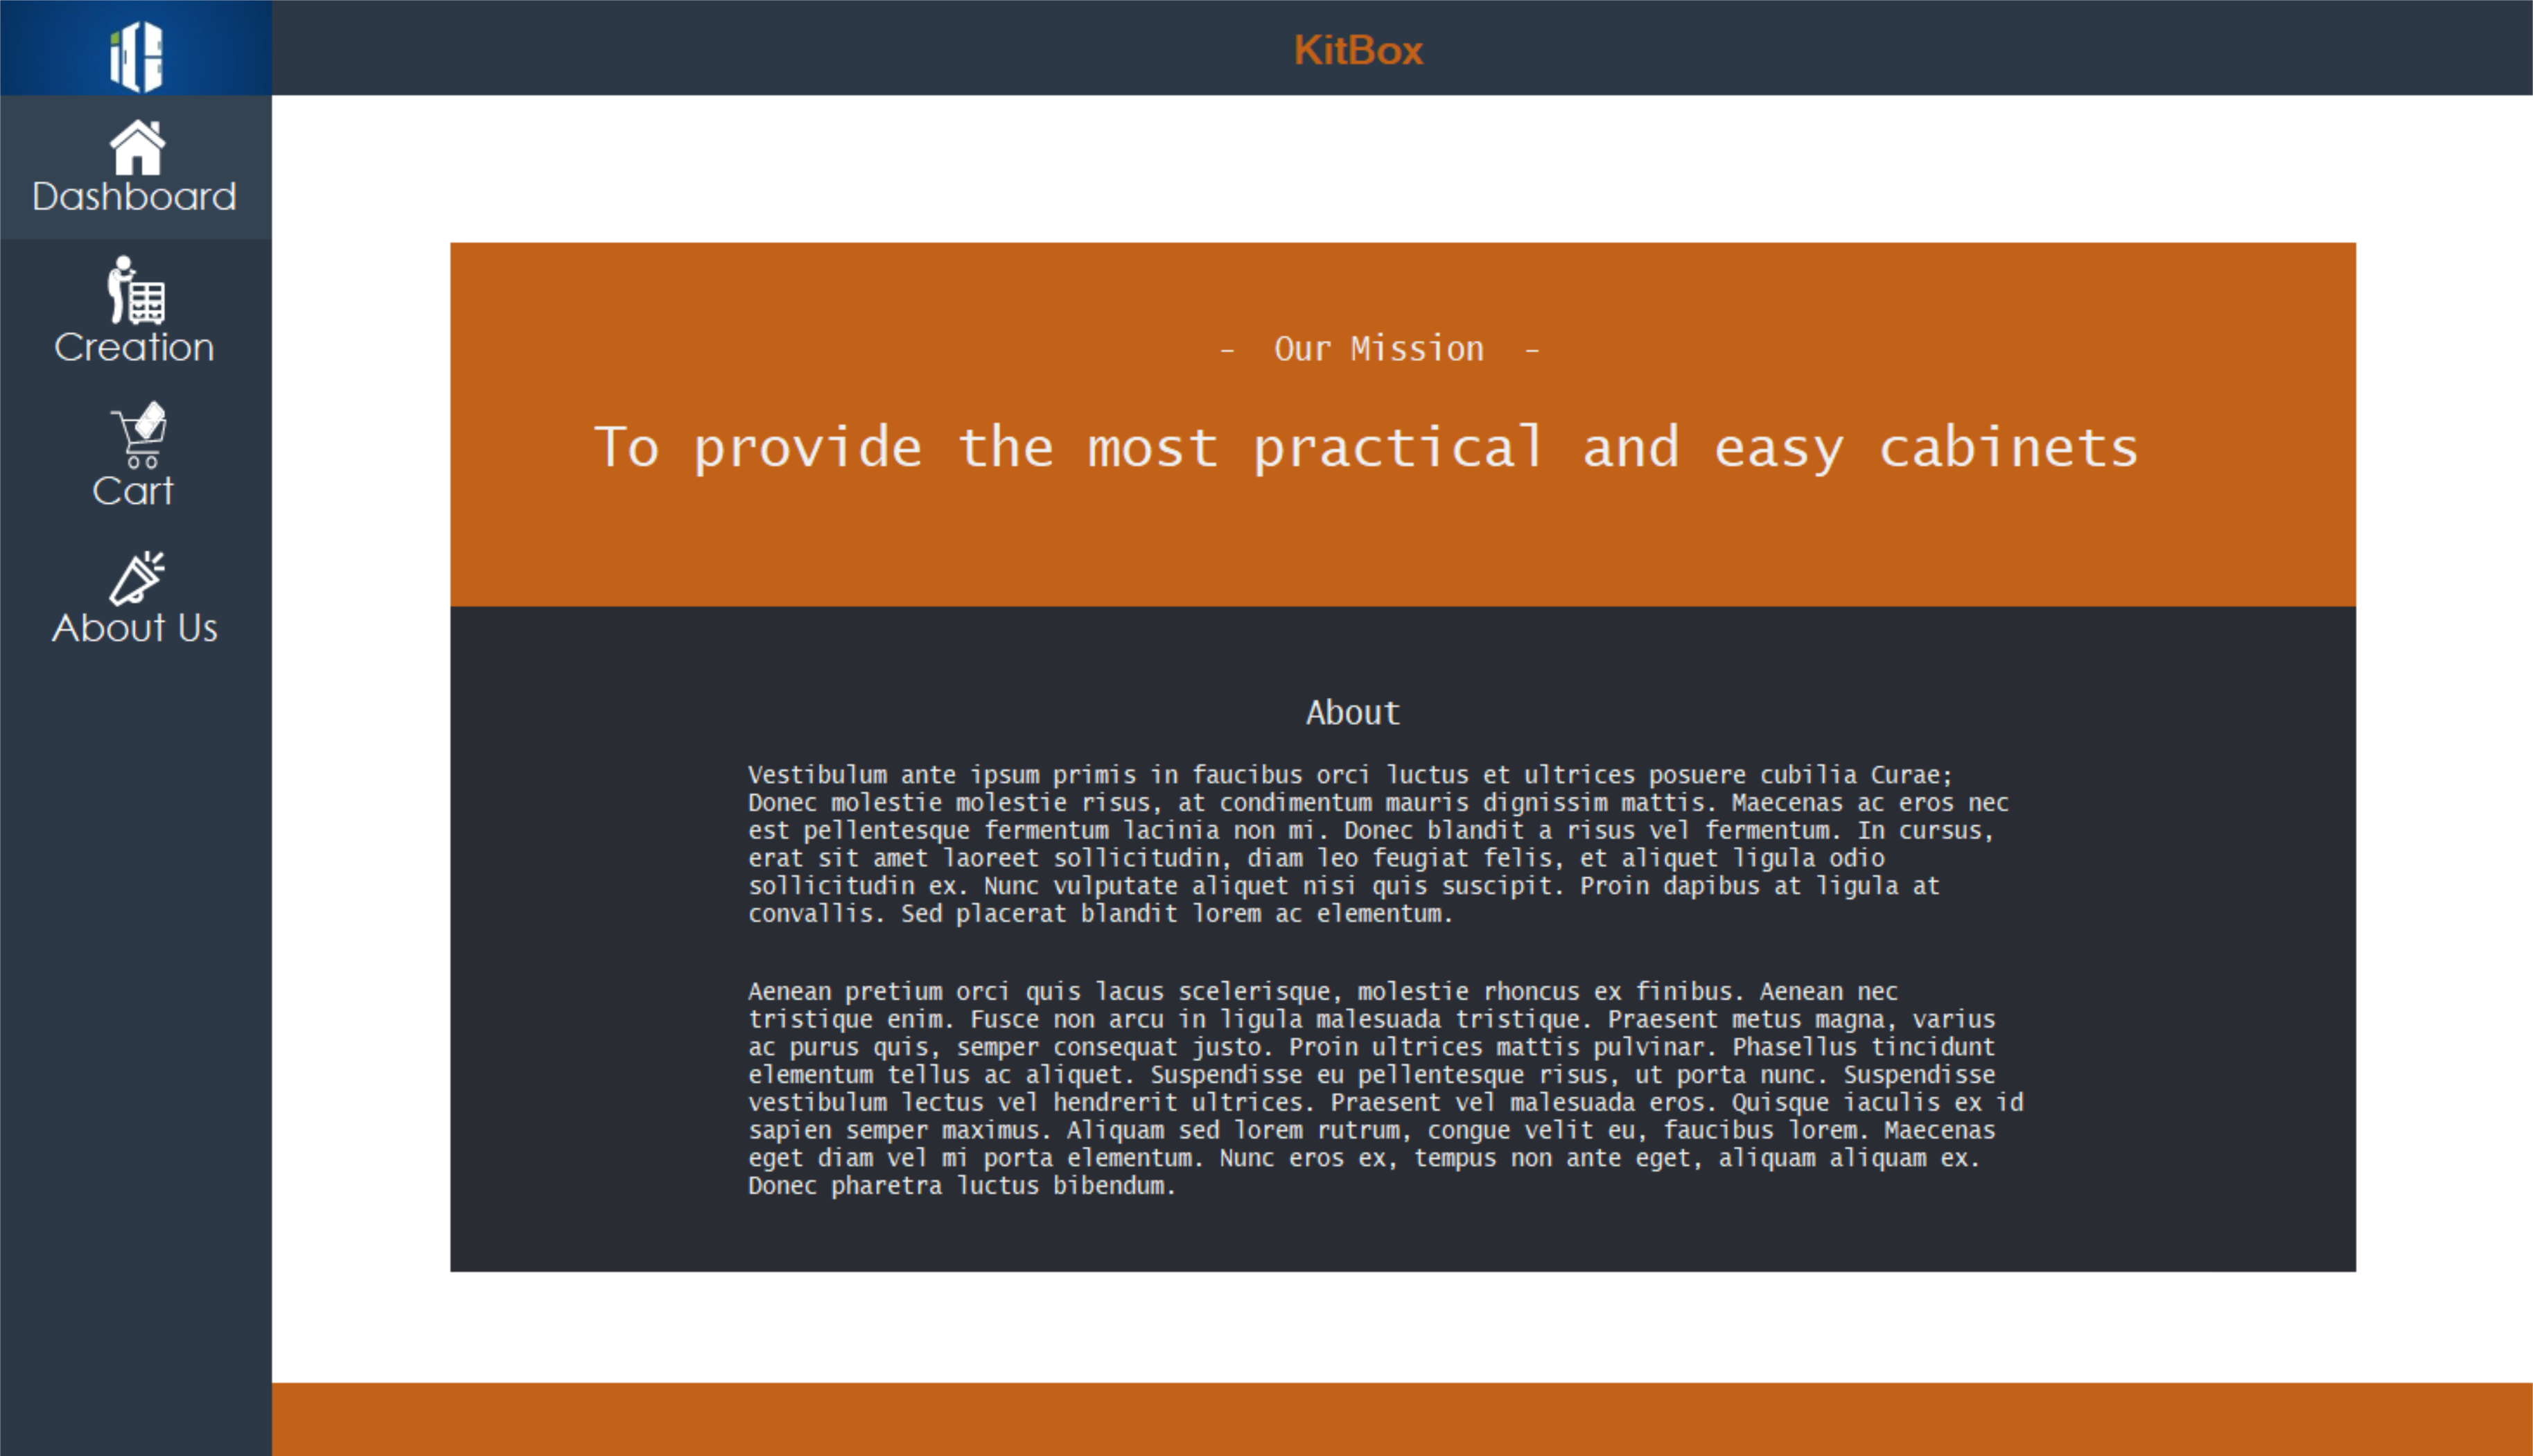
\includegraphics[width =1.2\textwidth,angle = 90]{Figures/AboutUs.PNG}
    		\rule{35em}{0.5pt}
    		\caption{About Us page}
    		\label{aboutus}
    	\end{figure*}
    	\vfill

\newpage
\section{Storekeeper Interface}
\label{Storekeeperinterface}
    \subsection{Stock Manager Tab Interface}
        \vfill
        \begin{figure*}[h!]
            \centering
    		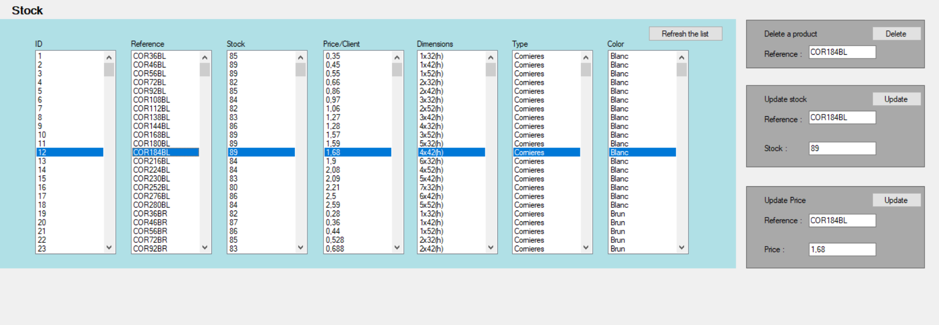
\includegraphics[width =1.2\textwidth,angle = 90]{Figures/StockManagerTab.png}
    		\rule{35em}{0.5pt}
    		\caption{Stock Manager Interface}
    		\label{stocktab}
    	\end{figure*}
    	\vfill
    	
	\newpage
	\subsection{New Product or Supplier Tab Interface}
    	\vfill
        \begin{figure*}[h!]
            \centering
    		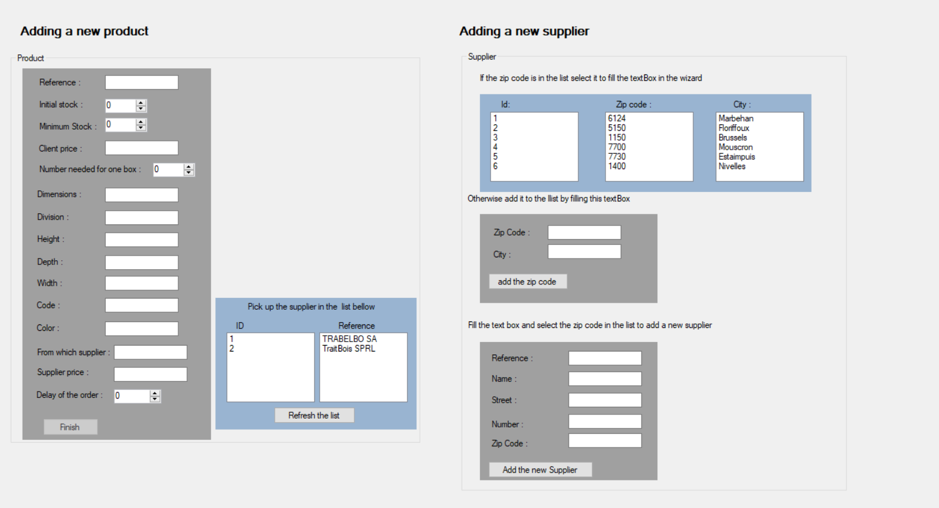
\includegraphics[width =1.2\textwidth,angle = 90]{Figures/SupplierTab.png}
    		\rule{35em}{0.5pt}
    		\caption{New Product and Supplier Interface}
    		\label{suppliertab}
    	\end{figure*}
    	\vfill
    	
	\newpage
	\subsection{Order Tab Interface}
    	\vfill
        \begin{figure*}[h!]
            \centering
    		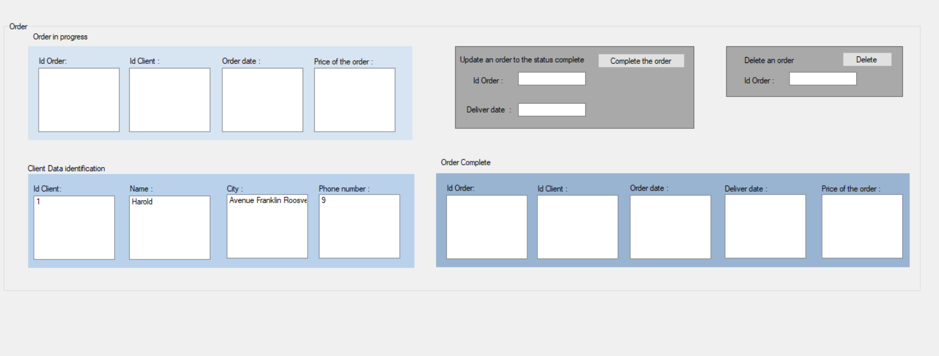
\includegraphics[width =1.2\textwidth,angle = 90]{Figures/OrderTab.png}
    		\rule{35em}{0.5pt}
    		\caption{Order Interface}
    		\label{ordermanagertab}
    	\end{figure*}
    	\vfill
    	
	\newpage
	\subsection{Client Tab Interface}
    	\vfill
        \begin{figure*}[h!]
            \centering
    		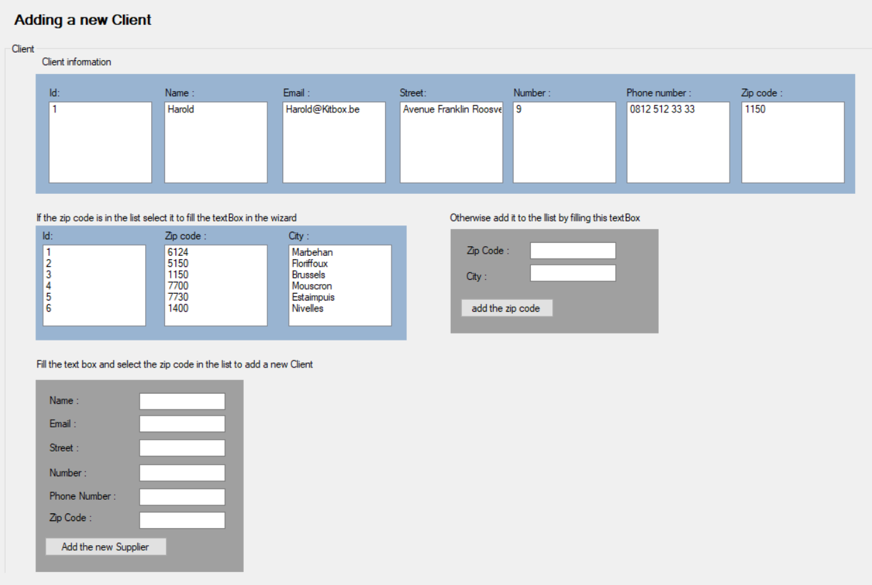
\includegraphics[width =1.2\textwidth,angle = 90]{Figures/ClientTab.png}
    		\rule{35em}{0.5pt}
    		\caption{Interface where you can find the customer's information}
    		\label{clientmanagertab}
    	\end{figure*}
    	\vfill